\documentclass[12pt,oneside,a4paper]{article}
\usepackage[utf8]{inputenc}
\usepackage[T1]{fontenc}
\usepackage[hungarian]{babel}
\usepackage{graphicx}
\usepackage{amsmath}
\usepackage{glossaries}
\usepackage{hyperref}
\usepackage{fancyhdr}
\usepackage{enumitem}
\usepackage[headheight=15mm, footskip=10mm]{geometry}
\usepackage{makeidx}
\usepackage{url}
\usepackage{times}
\usepackage[printonlyused,withpage]{acronym}
\usepackage{tikz}
\usepackage{tabularx}
\usepackage{pdfpages}
\usepackage{wrapfig}

\newcommand{\newsection}[1]{\clearpage\section{#1}}\label{makro}
\newcommand*{\titletext}{Yolov8-as szegmentációs háló és annak magyarázhatósága EigenCAM típusú modellfüggő magyarázó rendszerrel}

\usepackage{amsthm}

\theoremstyle{remark}
\newtheorem*{remarkth}{Válasz: \newline}
\newtheorem*{observation}{ \newline \textit}
\newenvironment{remark}{\begin{remarkth}}{\end{remarkth}}
\newcommand{\oldh}{\( "old" \)}\label{makro2}
\newcommand{\newh}{\( "new" \)}

\newenvironment{kerdes}{
    \medskip%
    \par\noindent\ignorespaces%
    \textit{\textsc{\textbf{Kérdés: }}}%
    \medskip
    \textsf%
}{%
\medskip
}

\makeindex
\makeglossaries

\newglossaryentry{Yolo}
{
    name=You Only Look Once,
    short=YOLO,
    description={You Only Look Once, egy gyors és hatékony objektumdetektáló neurális hálózat}
}
\newglossaryentry{Yolov8}{
short=YOLOv8,
name=You Only Look Once version 8,
description={A YOLOv8 egy hatékony és népszerű szemantikus szegmentációs hálózatcsalád legújjabb példánya}
}

\newglossaryentry{feature}
{
    name={feature},
    description={A feature egy adott kép vagy adat egyik jellemzője, amelyet a modell felhasznál a döntéshozatalhoz}
}

\newglossaryentry{EigenCAM}{
name=Eigen Class Activation Mapping,
short=EigenCAM,
description={Egy modellfüggő magyarázó rendszer, amely képes vizualizálni, hogy a mély tanuló hálózatok mely részei járultak hozzá a döntéshozatalhoz}
}
\newglossaryentry{Yolov5}{
short=YOLOv5,
name=You Only Look Once version 5,
description={A YOLOv5 egy hatékony és népszerű objektumdetektáló neurális hálózat}
}
\newglossaryentry{Inference}{
name=Inference,
description={Az inferencia a gépi tanulásban a modell által megtanult minták alkalmazását jelenti új adatokon}
}
\newglossaryentry{epoch}{
name=epoch,
description={Az Epochok száma adja meg hányszor megy végig a tanulás során a hűló a teljes adathalmazon}
}
\title{\titletext}
\author{Nyilas Péter}
\date{\today}



\pagestyle{fancy}
\fancyhf{}

% Header
\fancyhead[L]{
    
\includegraphics[width=4cm]{BMElogo}
}
\fancyhead[R]{
    
\includegraphics[width=1cm]{MITlogo}
}
\renewcommand{\footrulewidth}{0.4pt}
\pagestyle{fancy}

% Footer
\fancyfoot[L]{
    \footnotesize
    Budapest Műszaki és Gazdaságtudományi Egyetem \\
    Villamosmérnöki és Informatikai Kar \\
    Méréstechnikai és Információs Rendszerek Tanszék \\
    \url{www.mit.bme.hu}
}
\fancyfoot[R]{
    \raisebox{-0.9\height}{
\includegraphics[width=0.9cm]{viklogo}}
    \thepage
}

\makeglossary

\begin{document}

\maketitle
\newpage
\tableofcontents\label{ossz:tartalomjegyzek}
\newpage
\newsection{Bevezetés}\label{sec:bevezetes}
\pagestyle{fancy}
    Közlekedési objektumok detektálásával foglalkoztam a tavalyi témalaboratóriumomban,
     gépi látás (\ac{CV}) témakörében, mindezt Yolo architektúrájú neurális hálóval.
    Akkor a \glsentryshort{Yolov5}-tel foglalkoztam hagyományos keretes adatreprezentáció mellett és a dolgozatom végén
     haladási tervet fogalmaztam meg azért, hogy jobban elmerüljek ebben a területben.
Ezek akkor az alábbiak voltak:
\begin{enumerate}[label=\alph*., start=1]\label{enum:tervek}
    \item újabb hálóarchitektúra vagy nagyobb háló alkalmazása
    \item áttérni a szemantikus szegmentációs objektumreprezentációra a bounding box alapúról
    \item új (hardveres) erőforrás és jobb szoftveres kiszolgálás beszerzése és felépítése
\end{enumerate}
A két félév között viszont megismerkedtem a modellmagyarázási módszerekkel így hozzáadódott az alábbi pont:
\begin{enumerate}[label=\alph*., start=4]
    \item a háló döntéseit milyen magyarázó módszer mellett tudnám lehető legérthetőbben megjeleníteni és ezáltal megérthetővé tenni.
\end{enumerate}

    Előző féléves szakmai gyakorlatomban, képfeldolgozó neurális hálókkal dolgoztam.
    Itt feladatom volt megismerkedni az adatfeldolgozással, MLOps-al is ami, a mesterséges intelligenciával segített szoftverek kiszolgálását
    és fejlesztését könnyíti.
    Ekkor szembesültem azzal, hogy a neurális hálók azonban gyakran fekete dobozként (blackbox) működnek,
    ami komplikálttá teszi azok megértését.
    Azért, hogy biztonságosabbnak tudhassuk ezeket
    és megértésükkel későbbi hibáikat kijavíthassuk, fontos interpretálhatóság.
    Az interpretálhatóság nem más mint a modell döntéseinek megértése
    és magyarázata, ami kulcsfontosságú ezen modellek elfogadhatóságában és alkalmazhatóságában.

    A YOLOv8 (\gls{Yolov8}) egy népszerű és hatékony konvolúciós neurális háló.
    Ennek a szegmentációs változatát használom (Yolov8m\_seg), ez
    például objektumfelismerésre és objektum-klasszifikációra is tökéletesen használható.
    A modell architektúrája ismeretében betekinthetünk majd valamilyen külső eszközzel a héjjai közé,
    és megpróbálhatjuk megérteni a héjjak (layerek) közötti aktivációs függvények kimenetei alapján, a háló viselkedését.

    Egy ilyen eszköz az \glsentryshort{EigenCAM} (\gls{EigenCAM}) ami egy modellfüggő és gradiensmentes magyarázó rendszer,
    amely képes vizualizálni, hogy a mély tanuló hálózatok mely részei járultak hozzá a döntéshozatalhoz.
    Ehhez pedig
    az aktivációs függvények értékeit kiemeli a háló héjjaiból és a bemeneti képre vetíti ezeket, majd kombinálja
    ezt a mátrixot és az eredeti képet eggyé, megmutatva azt, hogy a kép mely részei milyen fontosak a döntések meghozásában.

\newsection{Mély tanulás és interpretálhatóság}\label{sec:mely-tanulas-es-interpretalhatosag}
A mesterséges intelligenciát tartalmazó szoftvereket azért használjuk gyakran, hogy rugalmasabb megoldást adjon akár
nehezen algoritmizálható problémáinkra is.
Azonban ezek működése nehezen nevezhető zártnak és kauzálisnak.
 Ezért elengedhetetlen az interpretálhatóság, vagyis annak képessége, hogy a modellek
döntéseit érthető és ésszerű módon magyarázza meg.
    Különböző magyarázó módszerek léteznek a mély tanulási modellek interpretálhatóságának növelésére.

\subsection{Magyarázhatóság}\label{subsec:magyarazhatosag}
A gépi tanulásban használt magyarázó módszerek két fő kategóriára oszthatók: modellfüggő és modellfüggetlen.
A modellfüggő magyarázó módszerek közvetlenül figyelembe veszik a modellek belső szerkezetét és működését a magyarázatok
létrehozásában.
Ezek a módszerek arra törekednek, hogy feltárják a modell döntéshozatali folyamatainak mechanizmusait és az
egyes predikciók alapját.
Például a gradiens visszaszármaztatás, osztály-aktivációs térképek(\ref{sec:eigencam:-modellfuggo-magyarazo}\label{sechiv}
és a LIME modellfüggő magyarázó módszerek.

Azomban a modellfüggetlen magyarázó módszerek általánosabb megközelítést alkalmaznak az interpretálhatóságra.
Ezek a módszerek nem igénylik a modell belső szerkezetének ismeretét a magyarázat létrehozásához, és általában
a bemeneti adatok és a modell predikciói közötti kapcsolatokat vizsgálják.
Például a perturbációs alapú módszerek, mint például a SHAP és a LIME együttes használata.


\begin{kerdes}
    Miért is ilyen fontos a modell interpretálhatósága és a magyarázhatósága?
\end{kerdes}
\begin{remark}
    Különösen fontos a jogi szabályozásban, hogy bármilyen szoftver-termék használatakor a döntések átláthatóak és
    érthetőek legyenek.
    Például az \ac{EU} által 2016-ban életbe léptetett Általános Adatvédelmi Rendelet (\ac{GDPR}) előírja, hogy az
    automatizált döntéshozatalnak átláthatónak kell lennie, és az érintetteknek joguk van tudni, hogy egy algoritmus
    milyen döntéseket hoz róluk.
\end{remark}
\newsection{YOLOv8: Szemantikus szegmentációs háló és működése}\label{sec:yolov8:-szemantikus-szegmentacios-halo}
    \begin{wrapfigure}{l}{0.2\textwidth}
        \centering
        
\includegraphics[width=0.2\textwidth]{Ultralytics}
        \caption{Ultralytics logo}
        \label{fig:Ultralytics}
    \end{wrapfigure}
    A YOLOv8 (\cite{Yolov8})\label{irodalomhivatkozas} egy hatékony és népszerű osztályozó és detektáló neurális
    hálózatcsalád legújabb példánya, amelyet számos számítógépes látás (\ac{CV})
    feladatban használnak.
    A \(""\)\gls{Yolo}\(""\) (\glsentryshort{Yolo}) megközelítést alkalmazza,
    amely gyors és pontos objektumdetektálást tesz lehetővé egyetlen neurális háló segítségével.


    A YOLOv8 működése során a bemeneti képet egyszer veszi figyelembe, és az objektumok pozícióját
    és osztályát egyetlen predikcióval határozza meg.
    Ez a modell különösen alkalmas valós
    idejű alkalmazásokhoz, mint például az önvezető járművek vagy a valós idejű videoelemzés.

    Ennek a hálónak én a szegmentációs változatát használtam, amely manapság egy eléggé új és népszerű
    irány a közlekedési objektumok detektálásában.
    Eddig ugyanis inkább 2--3 dimenziós ún. \("\)bounding boxokat\("\) azaz kereteket használtak a detektálni kívánt
    objektumok reprezentációjára, azonban a szegmentációs hálók képesek  ezeknek pontosabb azonosítására és
    lokalizációra.
    Az információ-gazdagabb  adatreprezentáció miatt, az objektumok pontos körvonalainak meghatározása lehetővé válik.
    Ezáltal a szegmentációs hálók pontosabb és részletesebb információkat nyújtanak az objektumokról,
    mint a keretes objektum-interpretáció.

\subsection{Yolov8 architektúra}\label{subsec:yolov8-architektura}
    A YOLOv8 egy képfeldolgozó (konvolúciós) mély neurális hálózat.
    Ami három különböző réteget használ a hálóarchitektúrában a képek feldolgozásához:
    \begin{itemize}
        \item konvolúciós rétegeket
        \item teljesen összekapcsolt rétegeket
        \item \("\)MaxPooling\("\) rétegeket,
    \end{itemize}

    A háló bemenetién a képet  konvolúciós és \("\)MaxPooling\("\) rétegeken keresztül feldolgozza,
    majd a kimeneti rétegekben meghatározza az objektumok pozícióját és osztályát, mindezt egy iteráció alatt,
    innen is jön a \("\)\gls{Yolo}\("\) elnevezés.
    A YOLOv8 architektúra~\ref{fig:Yolov8} általában három részre osztható:
    \begin{enumerate}
        \item Az előfeldolgozó rétegek, amelyek a bemeneti képet előkészítik a további feldolgozásra.
        \item A konvolúciós rétegek, amelyek a képet feldolgozzák és az objektumokat azonosítják.
        \item A kimeneti rétegek, amelyek meghatározzák az objektumok pozícióját és osztályát.
    \end{enumerate}
    \newpage
    \begin{figure}[ht]
        \centering
        \noindent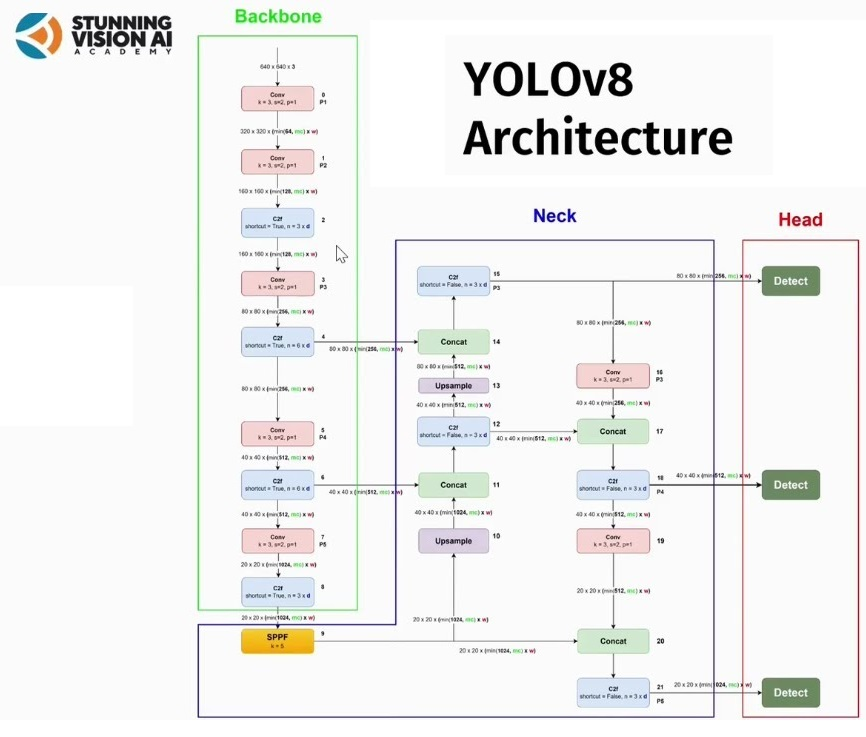
\includegraphics[width=1\linewidth]{maxresdefault}
        \label{fig:Yolov8}
    \end{figure}
    A YOLOv8 architektúra eltérő méretű és kapacitású változatokban érhető el, amelyek különböző feladatokhoz
    és alkalmazásokhoz használhatóak: (Attribútumok COCO adathalmaz alapján)
    \begin{table}[ht]
        \begin{tabularx}
        \textwidth{|X|X|X|X|}
            \hline
            \textbf{YOLOv8 verzió} & \textbf{Méret} & \textbf{Max. Pontosság (\ac{mAP})} & \textbf{Sebesség (\ac{ms})} \\
            \hline
            YOLOv8s & Kis & 37.3 & 0.99 \\
            \hline
            YOLOv8m & Közepes & 44.9 & 1.2 \\
            \hline
            YOLOv8l & Nagy & 50.2 & 2.39 \\
            \hline
            YOLOv8X & Hatalmas & 53.9 & 3.53 \\
            \hline
        \end{tabularx}\label{tab:Netsizes}
    \end{table}
    Ezenfelül beszélhetünk szegmentációs hálókról (bővebben: \aref{subsec:szemantikus-szegmentacio} alfejezetben) és
    hagyományosan a bounding boxokat detektáló hálókról, amik az objektumok köré illesztenek egy befogó minimális
    területű téglalapot/téglatestet.(Yolov8\_seg vs. Yolov8)

    Témalaboratórium alatt bounding box adatreprezentációjú neurális hálót használtam,
    most viszont, áttértem a szemantikus szegmentációra.
    Ennek okait a következő alfejezetben felsorolom.
\newpage

\subsection{Szemantikus szegmentáció}\label{subsec:szemantikus-szegmentacio}

A szemantikus szegmentáció\index{szemantikus szegmentáció} egy olyan adatreprezentációs forma, amelyben a cél az
objektumokat tartalmazó kép egyes részeinek (például pixeljeinek) címkézése az objektumokhoz tartozó osztályok szerint.
Van emellett egy másik szegmentációs adatreprezentációs forma, az ún. egyed szegmentáció\index[szemantikus szegmentáció]
{Egyedszegmentáció}, amelyben minden objektumot külön, azaz egyedenként kell detektálni és akár számon tartani (indexelni),
míg a szemantikus szegmentációban csak az objektumok osztályait kell meghatározni az egyed megkülönböztetése nélkül.
Más szavakkal, minden képpontot hozzá kell rendelni egy osztályhoz vagy kategóriához, például autó, biciklis, gyalogos stb.
Szakmai gyakorlatom során  eddig csak szemantikus szegmentációval foglalkoztam.
Amely módszer lehetővé teszi a \glsentryshort{Computer Vision} rendszereknek, hogy pontosan azonosítsák és lokalizálják az
objektumokat egy adott képen.

Tehát a szemantikus szegmentációt leírhatjuk úgy, ha egy képet jelölünk \(I\) -vel, akkor a szemantikus
szegmentáció pedig egy olyan függvény,\(F: I \rightarrow L\), ahol \(L\) a lehetséges osztályok halmaza, és \(F\) minden
képpontot hozzárendel egy osztályhoz, ez az osztály-hozzárendelés lesz a maszk.
A szemantikus szegmentáció kiemelt fontosságú az önvezető autók, a
videoelemzés, a térképek építése és sok más
alkalmazásban, ahol pontos és részletes objektum-felismerésre van szükség.
\begin{figure}[ht]
    \centering
    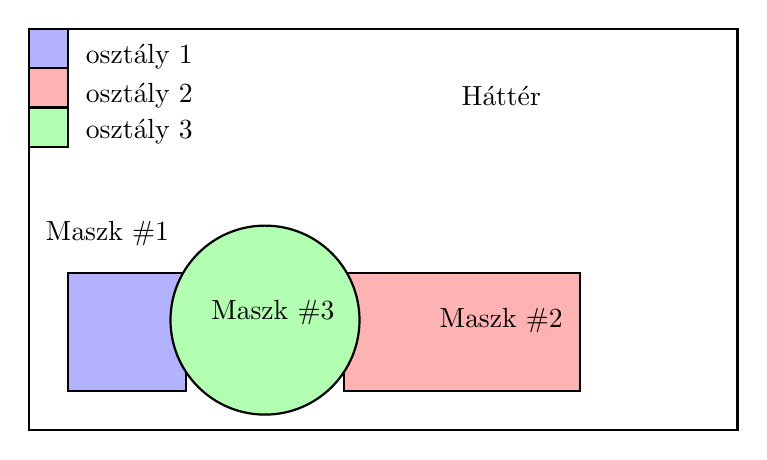
\begin{tikzpicture}
        \draw[thick] (0,0) rectangle (9,5.1);
        \node at (6,4.25) {Háttér};

        \draw[thick, fill=blue!30] (0.5,0.5) rectangle (2,2);
        \draw[thick, fill=red!30] (4,0.5) rectangle (7,2);
        \draw[thick, fill=green!30] (3,1.4) circle (1.2);
        \node at (1,2.5) {Maszk \#1};
        \node at (6,1.4) {Maszk \#2};
        \node at (3.1,1.5) {Maszk \#3};
        \draw[thick, fill=blue!30] (0,4.6) rectangle (0.5,5.1);
        \node[right] at (0.6,4.75) {osztály 1};
        \draw[thick, fill=red!30] (0,4.1) rectangle (0.5,4.6);
        \node[right] at (0.6,4.25) {osztály 2};
        \draw[thick, fill=green!30] (0,3.6) rectangle (0.5,4.1);
        \node[right] at (0.6,3.8) {osztály 3};
    \end{tikzpicture}
    \caption{szegmentáció példa}\label{fig:szegmentation example}
\end{figure}
Tehát az adatreprezentációs módszerváltást azért tartottam fontosnak:
\begin{enumerate}
    \item ,mert pontossága jóval felülmúlja az előző módszerét.
    \item ,mert az adathalmaz alapvetően szemantikus szegmentálási módszerrel van annotálva,
            kevés adat-előkészítési munkálat  szükséges.
    \item ,mert könnyebben érthető a feldolgozott kép, nincs olyan hogy az objektumok túlzott sűrűsége miatt túl sok
           doboz keletkezik ami megnehezíti vagy akár ellehetetlenítheti a kiolvasást.
\end{enumerate}


\subsection{Adathalmazok és kísérletek}\label{subsec:adathalmazok-es-kiserletek}
    Adathalmazként a témalaboratórium alatt végzett munkámhoz hasonlóan a CityScapes\index{CityScapes}
    (\url{https://www.cityscapes-dataset.com}) szemantikusan szegmentált adathalmazt, annak is a pontosan annotált
    (Fine Annotated),\aref{fig:CityScapes-Examples}\label{kephivatkozas}.képen bemutatott,
    adathalmazát használtam, ami osztályszegmentációs maszkokat biztosít az elérhető képekhez.
    Ezek a képek kicsit több mint 5000 városi közlekedési szituációt ábrázolnak
    németországi városokból.

    Ez az adathalmaz elég nagy varianciával rendelkezik számunkra ahhoz, hogy az adathalmazból egy
    robusztus szegmentációs hálót tudjunk tanítani közlekedési objektumok detektálására és osztályozására.


    \begin{figure}[ht]
       \centering
        \noindent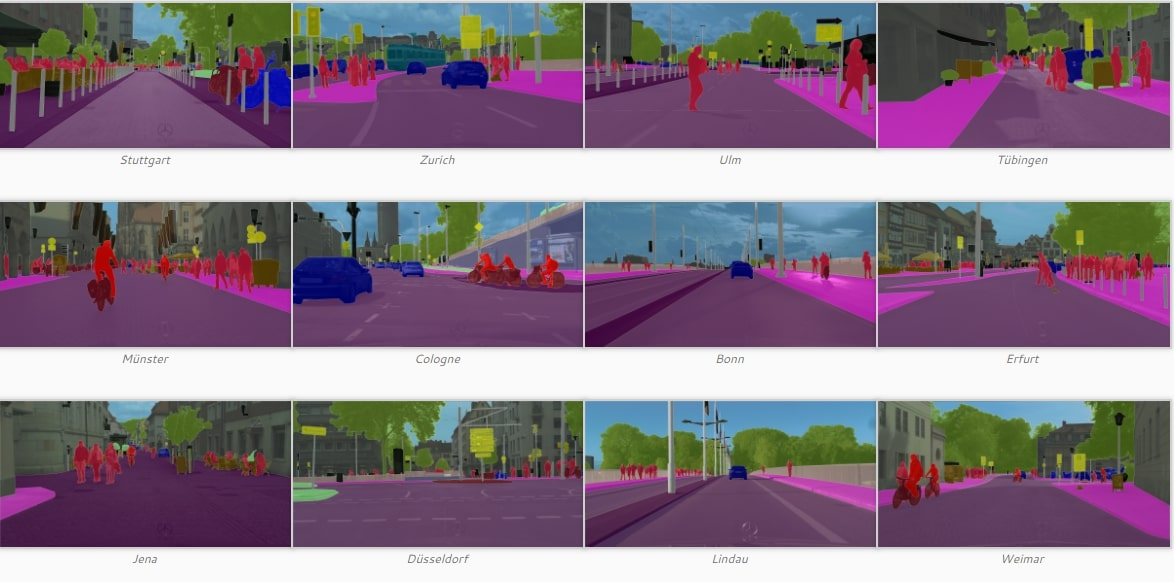
\includegraphics[width=1\linewidth]{cityscapes}
        \caption{CityScapes Examples}
        \label{fig:CityScapes-Examples}
    \end{figure}
    A tanításhoz és validációhoz a maszkokat poligonok formájában kaptam meg szöveges (.yaml) formában, ezeket a poligonokat
    minimális átalakítás után be is tudtam adni a háló bemenetére a megfelelő képekhez rendelve (szegmentációs
    maszkokról:~\ref{subsec:szemantikus-szegmentacio}. oldalon értekezek.)
    A kísérletek:~\ref{tab:Activations} táblázatban találhatóak.

    A magyarázat a kísérletekhez a ~\pageref{subsec:magyarazat}\label{pageref}.
    oldalon található.

    Ezeket az adatokat használom a későbbiekben arra, hogy megpróbáljuk megérteni a hálónkat az aktivációs függvényeinek kimenetei
    alapján.
    Ezeket a teszteket amiket az \glsentryshort{EigenCAM}\index{EigenCAM}-mal végeztem, a németországi Bonn városában
    vették fel és mivel a teszt-halmaz része, így a háló tanításban és a validációban eddig nem szerepelt.
\subsection{MLOps}\label{subsec:mlops}
A háló tanításához és validálásához használtam egy online kiértékelő, és eredményösszesítő felületet, ez pedig a Comet.ml\index{Comet} online platform ("alternatívája a Weights \& Biases"-nek), amely egy Github fiókhoz rendelve, segít a \ac{ML} projektek adminisztrációjában.
A Comet.ml (\url{https://www.comet.ml}) egy kollaboratív \ac{MLOps} platform, amely lehetővé teszi, hogy könnyen és
    hatékonyan figyelhessük a futó tanításainkat, validációinkat és \gls{Inference}inket.
    Számos funkciót kínál:
    \begin{itemize}
        \item Rögzíti és követi a kísérletek metrikáit, hiperparamétereit, modellváltozatokat és naplófájljait.
        \item Különböző diagramok és grafikonok segítségével jeleníti meg és elemzi az adatokat és az eredményeket.
        \item Lehetőséget ad a különböző kísérletek összehasonlítására és megosztására, akár csapatmunkára is használható.
        \item Automatikusan rögzíti és követi a modell változásait és fejlődését a tanítás folyamán az idő múlásával.
        \item Integrálható más keretrendszerekkel és eszközökkel, és rendelkezik egy API-val is, amely lehetővé teszi a platform
            saját igényeiknek megfelelő testreszabását.
    \end{itemize}
    \begin{observation}
        Összességében a Comet.ml egy teljes körű platform, amely segíti a \ac{ML} hatékony kezelését
        és nyomon követését, valamint lehetővé teszi a felhasználók számára, hogy gyorsabban és hatékonyabban dolgozzanak
        valamint jobban manageljék kísérleteiket.
    \end{observation}

\newsection{EigenCAM: Modellfüggőn magyarázó}\label{sec:eigencam:-modellfuggo-magyarazo}
     Az \glsentryshort{EigenCAM}\index{EigenCAM} (Eigen Class Activation Mapping) egy modellfüggő magyarázó módszer (forrás~\cite{pytorch-grad-cam}:), amelyet a mély tanulási
     modellek interpretálhatóságának növelésére fejlesztettek ki.
     Célja, hogy vizualizálja és magyarázza meg a modellek döntéseit a bemeneti adatok alapján,
     osztály-diszkrimináció nélkül, tehát ebben az esetben nem lesznek külön osztályokra szedve az aktivációk, hanem az
     összes osztály átlagos aktivációját kapjuk meg.

    Az \glsentryshort{EigenCAM} működése során az algoritmus végiglépked a háló kiválasztott héjain és kiértékeli
     az aktivációs függvények mátrixát.
    Ezt a mátrixot kiterjeszti (ha kell) annak a képnek méretére amire éppen az \gls{Inference}et futtatjuk.
    (forrás~\cite{muhammad2020eigencam}:)
    Az ez által generált \("\)hőtérkép\("\) (Heatmap) már jó esetben lehetővé teszi azt, hogy közelebb kerüljünk
     annak megértéséhez, hogy a kép mely tartományai játszanak nagyobb szerepet a detekcióban és klasszifikációban.

     Azonban fontos tudni, hogy az \glsentryshort{EigenCAM} csak egy interpretálhatósági eszköz, és nem biztosít teljes képet
     a modell működéséről.
     Ugyanis ezek az eszközök csak a hálónak egy szeletébe engednek betekintést nyerni, amik önmagukban nehezen értelmezhetőek.
     Sokszor ez nem is enged logikus következtetést levonni.

     Az aktivációs csoportok képenként újrarendeződnek így metszeteket is nehéz automatizáltan készíteni.
     Ez pedig elengedhetetlen annak érdekében hogy biztosra mondjuk egy következtetés magyarázását.

\subsection{Aktivációk}\label{subsec:activations}
Az aktivációs függvények a modell héjainka kimeneti függvényei ahol \("x\) az input, \("W"\) a súlymátrix és \("b"\) a
    \("\)bias\("\) vagyis eltolási vektor.
        Az utolsó héjban egy lineáris aktivációs(\ac{ReLU})~\eqref{eq:RELU}\label{alignhivatkozas} függvényt használunk,
    míg az összes többi héjban egy
    szivárgó rektifikált lineáris aktivációs függvényt(\ac{LReLu})~\eqref{eq:LRELU}\label{eqhivatkozas} használunk:
    \begin{equation}
        \text{ LReLu:}
    \varphi(x) = \begin{cases}
      x, & \text{ha } x > 0 \\
      0.1x, & \text{különben}
    \end{cases}\label{eq:LRELU}
    \end{equation}\label{eq:activation_functions}


    \begin{align}
    \text{ReLU:}
    \varphi(x)=\begin{cases}
      x, & \text{ha } x > 0 \\
      0, & \text{különben} \end{cases}\label{eq:RELU} \\
    \text{Sigmoid:}
    \varPhi(x) &= \frac{1}{1 + e^{-x}} \label{eq:Sigmoid}
    \end{align}

\newsection{Az EigenCAM alkalmazása a YOLOv8-ra}\label{sec:az-eigencam-alkalmazasa-a-yolov8-ra}
    Az \glsentryshort{EigenCAM}\index{EigenCAM} alkalmazása a YOLOv8 szemantikus szegmentációs hálóra lehetővé teszi számunkra,
     hogy megértsük miképpen azonosít és lokalizál objektuomokat képeken és videókon a modell.
    (\cite{YoloV8-CAM} alapján).

    Az \glsentryshort{EigenCAM} konkrét működési folyamata \aref{fig:flowchart}\label{abrahiv} ábrán látható.
    A CityScapes\index{CityScapes} adathalmazon tanítottuk a Yolov8m-seg hálót (ami egy közepes méretű Yolov8 szegmentáló háló)
    , majd az EigenCAM segítségével vizualizáltuk az aktivációkat,
    amelyeket a háló a képek feldolgozása közben produkál (ezt az EigenCAM adja a hálónak egy olyan folyamaton keresztül
    amit \gls{Inference}nek nevezünk).
    Ezeket az EigenCAM kivezeti és rávetíti a bemenő képre (ezt a folyamatot lásd
    \aref{fig:flowchart} képen és\aref{Inference} pontban \label{listahiv} ), a különböző
    héjak aktivációit külön-külön.
    Amikor végez a kép előállításával azt HEATMAP formájában az output mappájába helyezi.
    Ezeket a heatmapokat majd~\pageref{sec:magyarazhatosagi-eredmenyek-es-ertekeles}. oldalon láthatjuk.

\begin{center}
    \resizebox{1\textwidth}{!}{%
        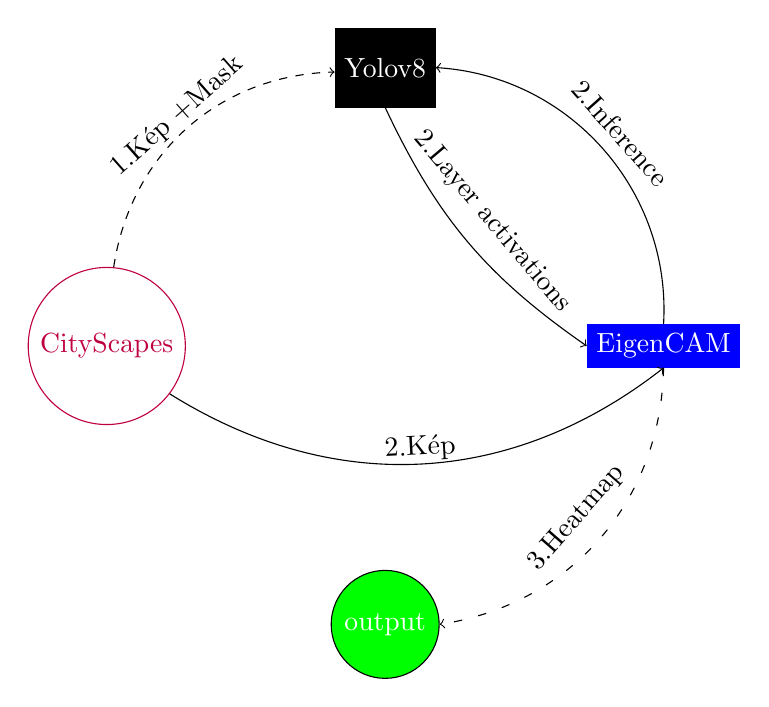
\begin{tikzpicture}
            \begin{scope} [node distance=5cm]
                \node[shape=circle, draw, color=purple] (CityScapes) {CityScapes};
                \node[shape=rectangle, draw, color=black, fill=black,
                    text=white, minimum height=1cm, minimum width=1cm] (Yolov8) [above right of=CityScapes] {Yolov8};
                \node[shape=rectangle, draw, color=blue, fill=blue, text=white] (EigenCAM) [below right of=Yolov8] {EigenCAM};
                \node[shape=circle, draw, fill=green,
                    text=white] (output) [below left of=EigenCAM] {output};
            \end{scope}
            \draw[->, dashed] (CityScapes) to [bend left=40] node [sloped, pos=0.5, yshift=0.2cm] {1.Kép +Mask} (Yolov8);
            \draw[->] (CityScapes) to [bend left=-35] node [sloped, pos=0.5, yshift=0.2cm] {2.Kép} (EigenCAM.south);
            \draw[->] (Yolov8.south) to [bend right=15] node [sloped, pos=0.5, yshift=0.4cm] {2.Layer activations} (EigenCAM.west);
            \draw[->] (EigenCAM.north) to [bend right=45] node [sloped, pos=0.5, yshift=0.3cm] {2.Inference} (Yolov8.east);
            \draw[->, loosely dashed] (EigenCAM.south) to [bend left=40] node [sloped, pos=0.5, yshift=0.4cm] {3.Heatmap} (output.east);
            \label{fig:flowchart}
        \end{tikzpicture}
    }

    \end{center}
\subsection{\Aref{fig:flowchart}.ábra jelmagyarázata}\label{subsec:aref{fig:flowchart}-jelmagyarazata}
\begin{itemize}\label{itemize}
        \item Normál Szaggatott: Tanítási időben.
        \item Teli nyíl: Inference (EigenCAM használata) közben.\label{Inference}
        \item Laza szaggatott nyíl: Inference idő után.
    \end{itemize}
\subsection{Implementáció lépései}\label{subsec:impelemntacio}
\begin{enumerate}
        \item Github és Comet repository létrehozása és felkonfigurálása
        \item Tanító, validációs és detektáló állományok megírása
        \item Adatfeldolgozás, és adatbázis-management
        \item Tanítás és validáció
        \item Modellanalízis
        \item Modellmagyarázó módszer bevetése
        \item Modellmagyarázó módszer kimenetének értékelés és magyarázata
\end{enumerate}
\begin{figure}[ht]
    \centering
    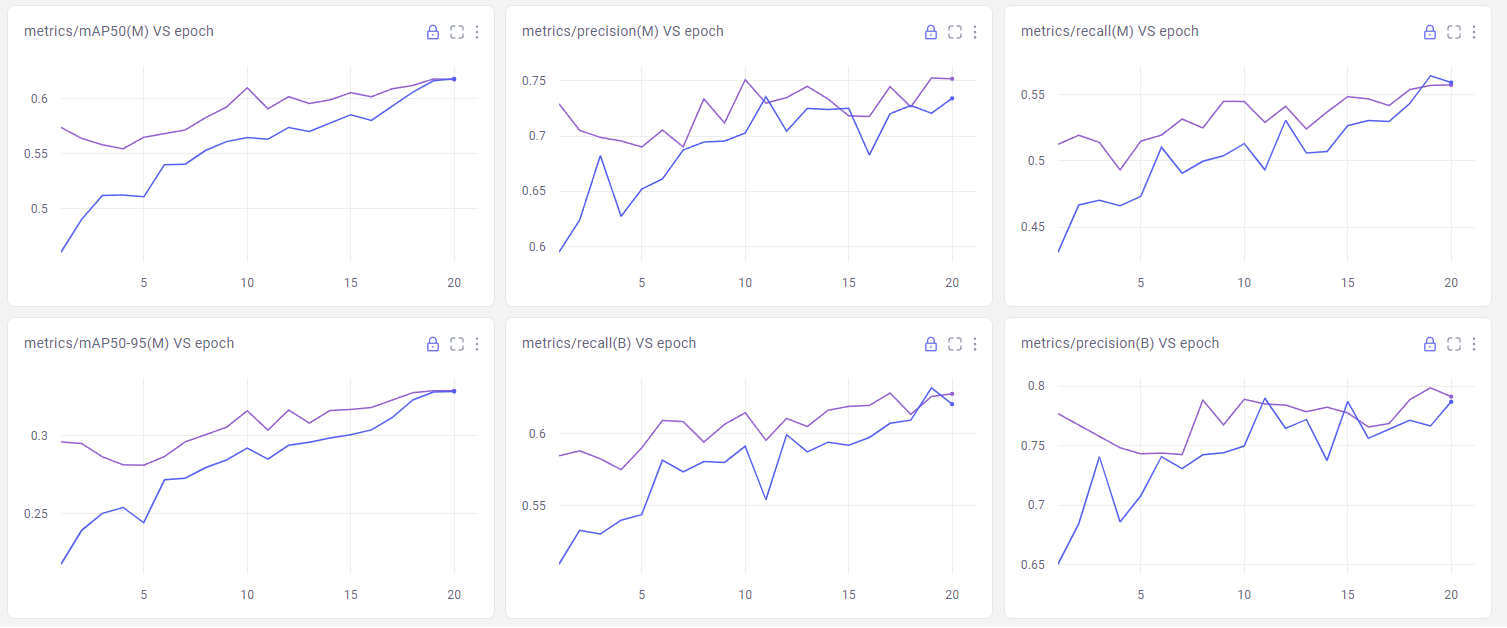
\includegraphics[width=1\linewidth]{modelltanitas}
    \caption{A tanítás folyamata}
    \label{fig:tanitas}
\end{figure}

\newsection{Magyarázhatósági eredmények és értékelés}\label{sec:magyarazhatosagi-eredmenyek-es-ertekeles}
    A két hálót, legyen az egyik \oldh\label{makrohasznalat} a másik \newh, \oldh egy yolov8m-seg háló 20
    \gls{epoch} keresztól tanult a ugyanazon teljes adathalmazon, a másik pedig 40 \gls{epoch} keresztül tanítottam.


    Az \glsentryshort{EigenCAM}\index{EigenCAM} által nyújtott kimenet amit ábrázoltam \aref{tab:Activations}
    táblázatban\label{hivatkozas}.
    A két háló detekciója alig különbözik.
    Kizárólag abban különböznek, hogy milyen bizonyosságban képesek megmondani átlagosan az objektumok osztályát.
    Ezért elegendőnek találtam a következőkben csak az \newh háló eredményeit tárgyalni.


\begin{table}[h!]

    \noindent\begin{tabular}{|p{0.05\textwidth}|c|c|c|}
        \hline
        \noindent Layer&\oldh & \newh & detection\\
        \hline
        -4.&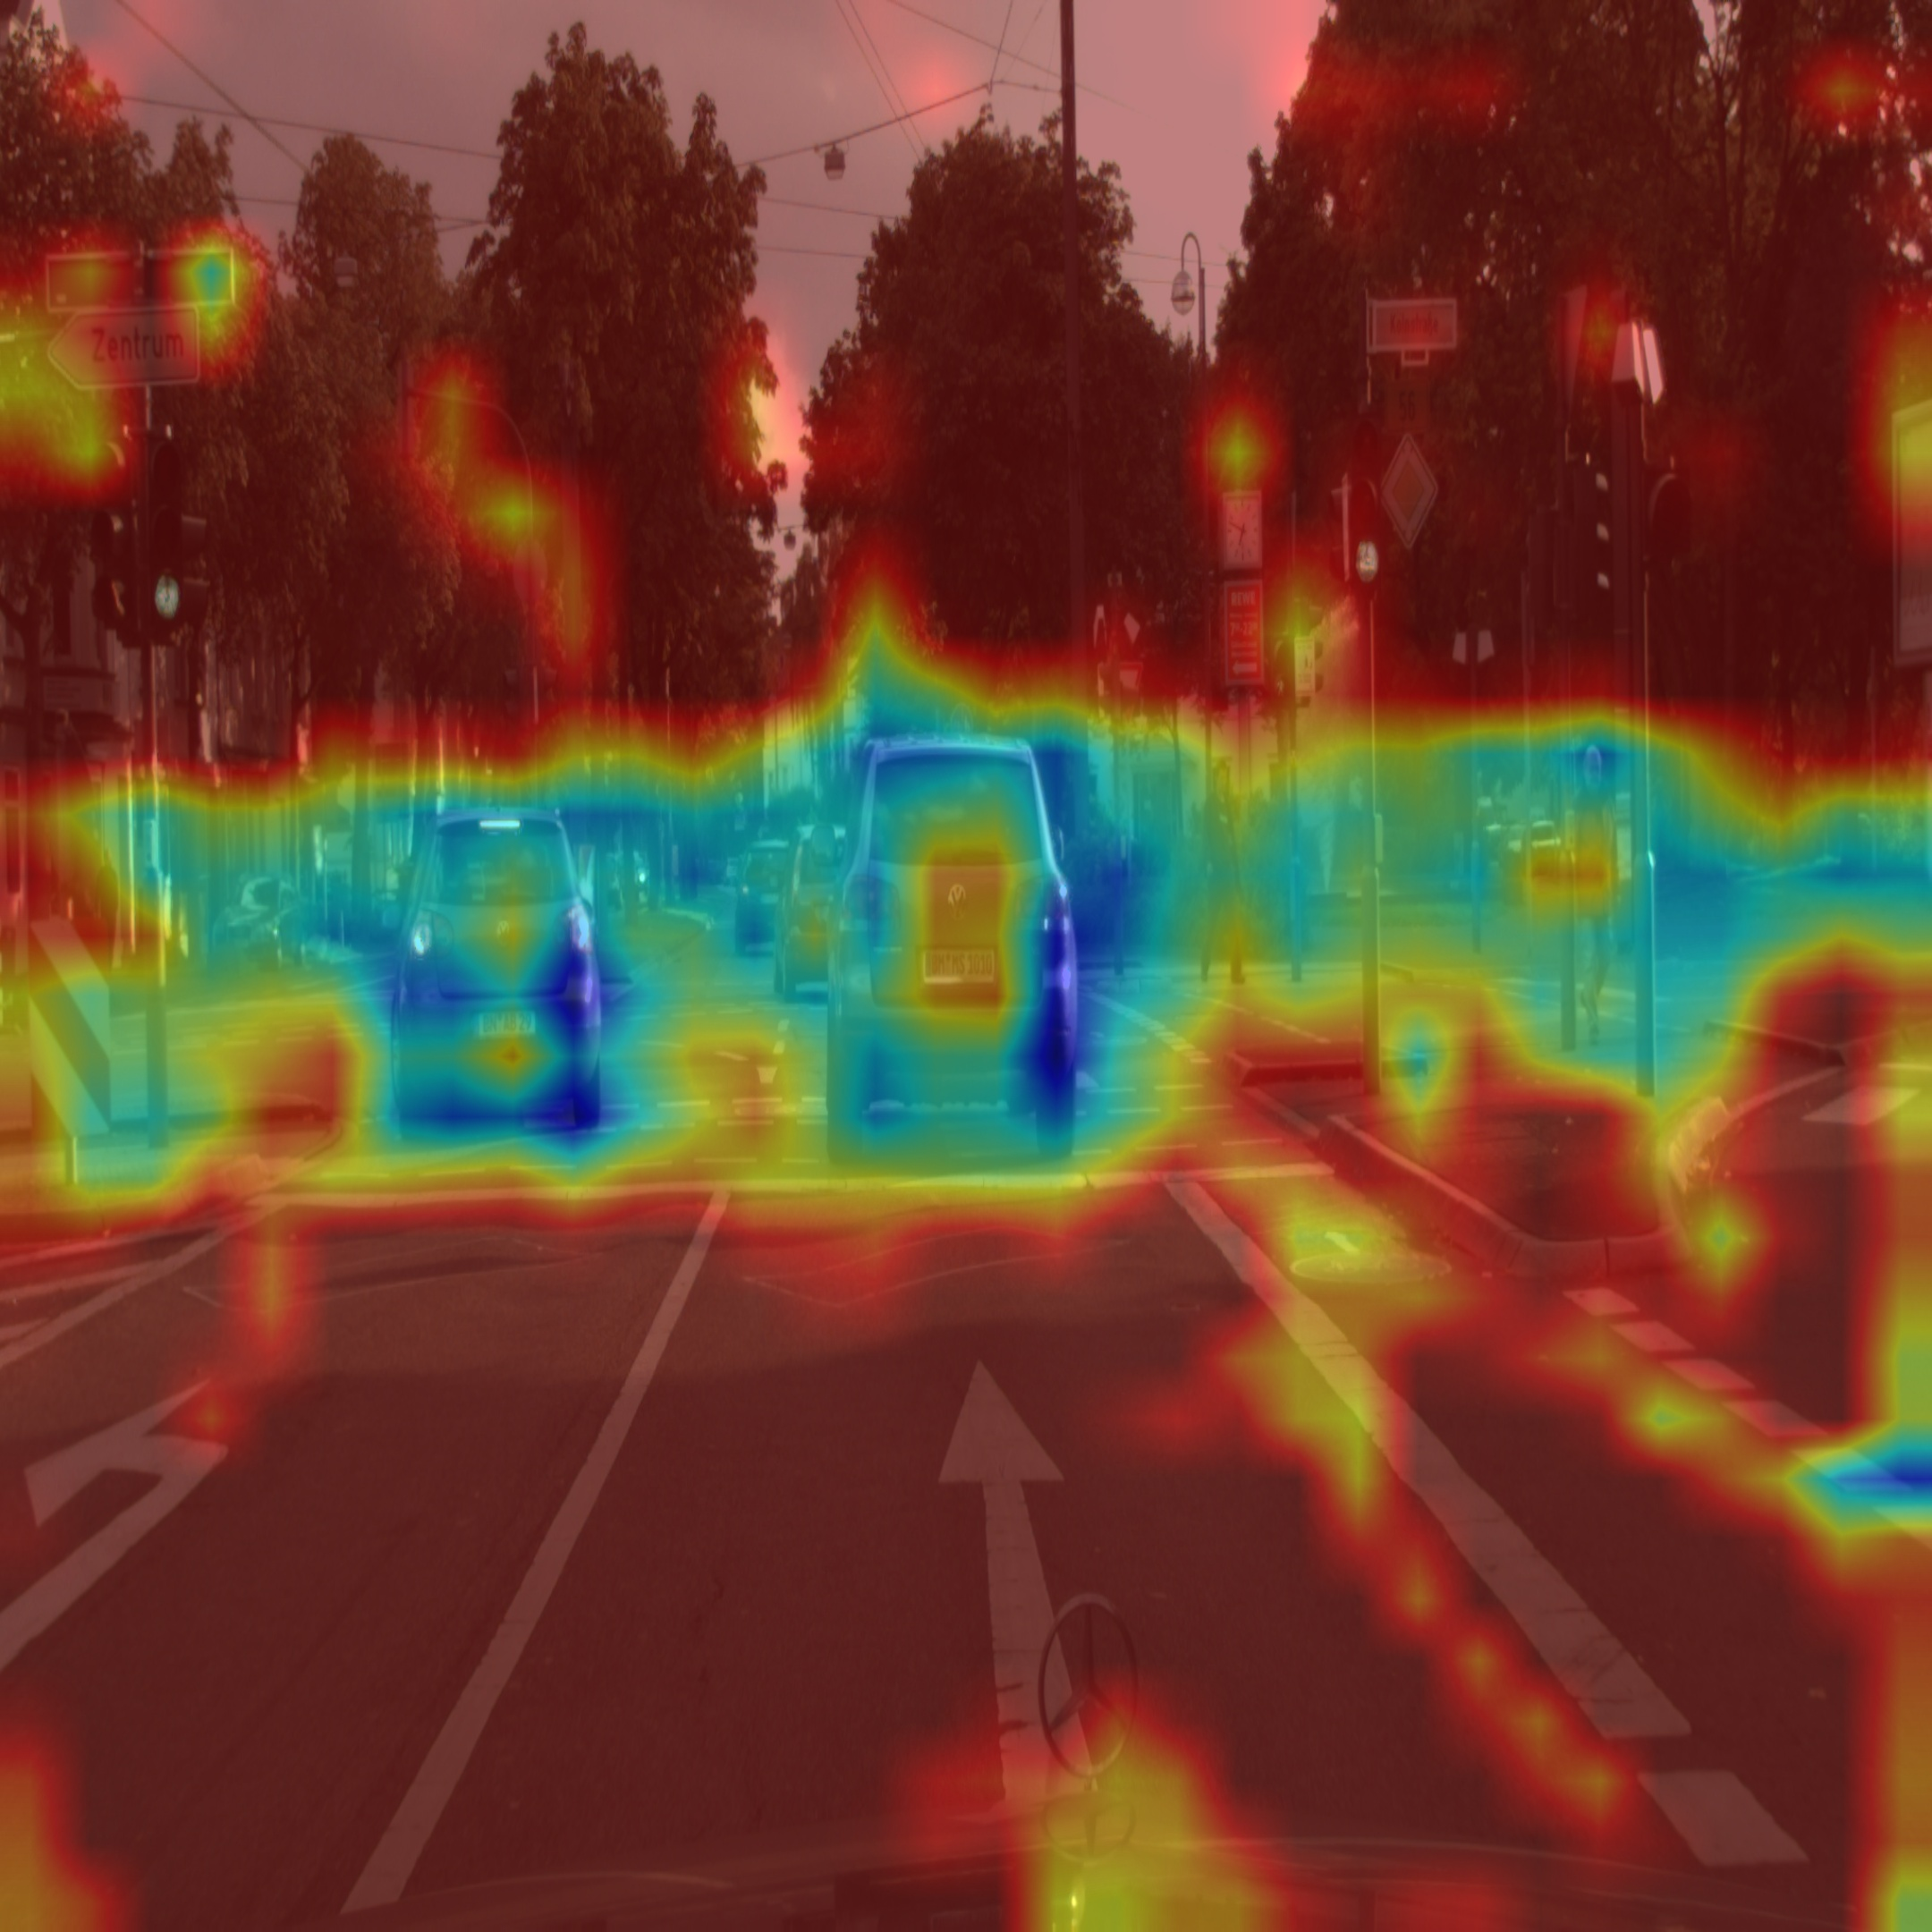
\includegraphics[width=0.316\textwidth]{old_layer-4} &
        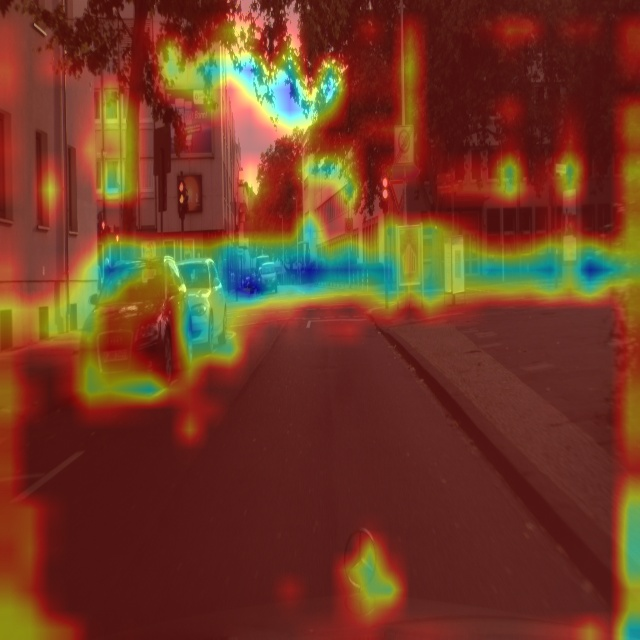
\includegraphics[width=0.316\textwidth]{new_l-4} &
        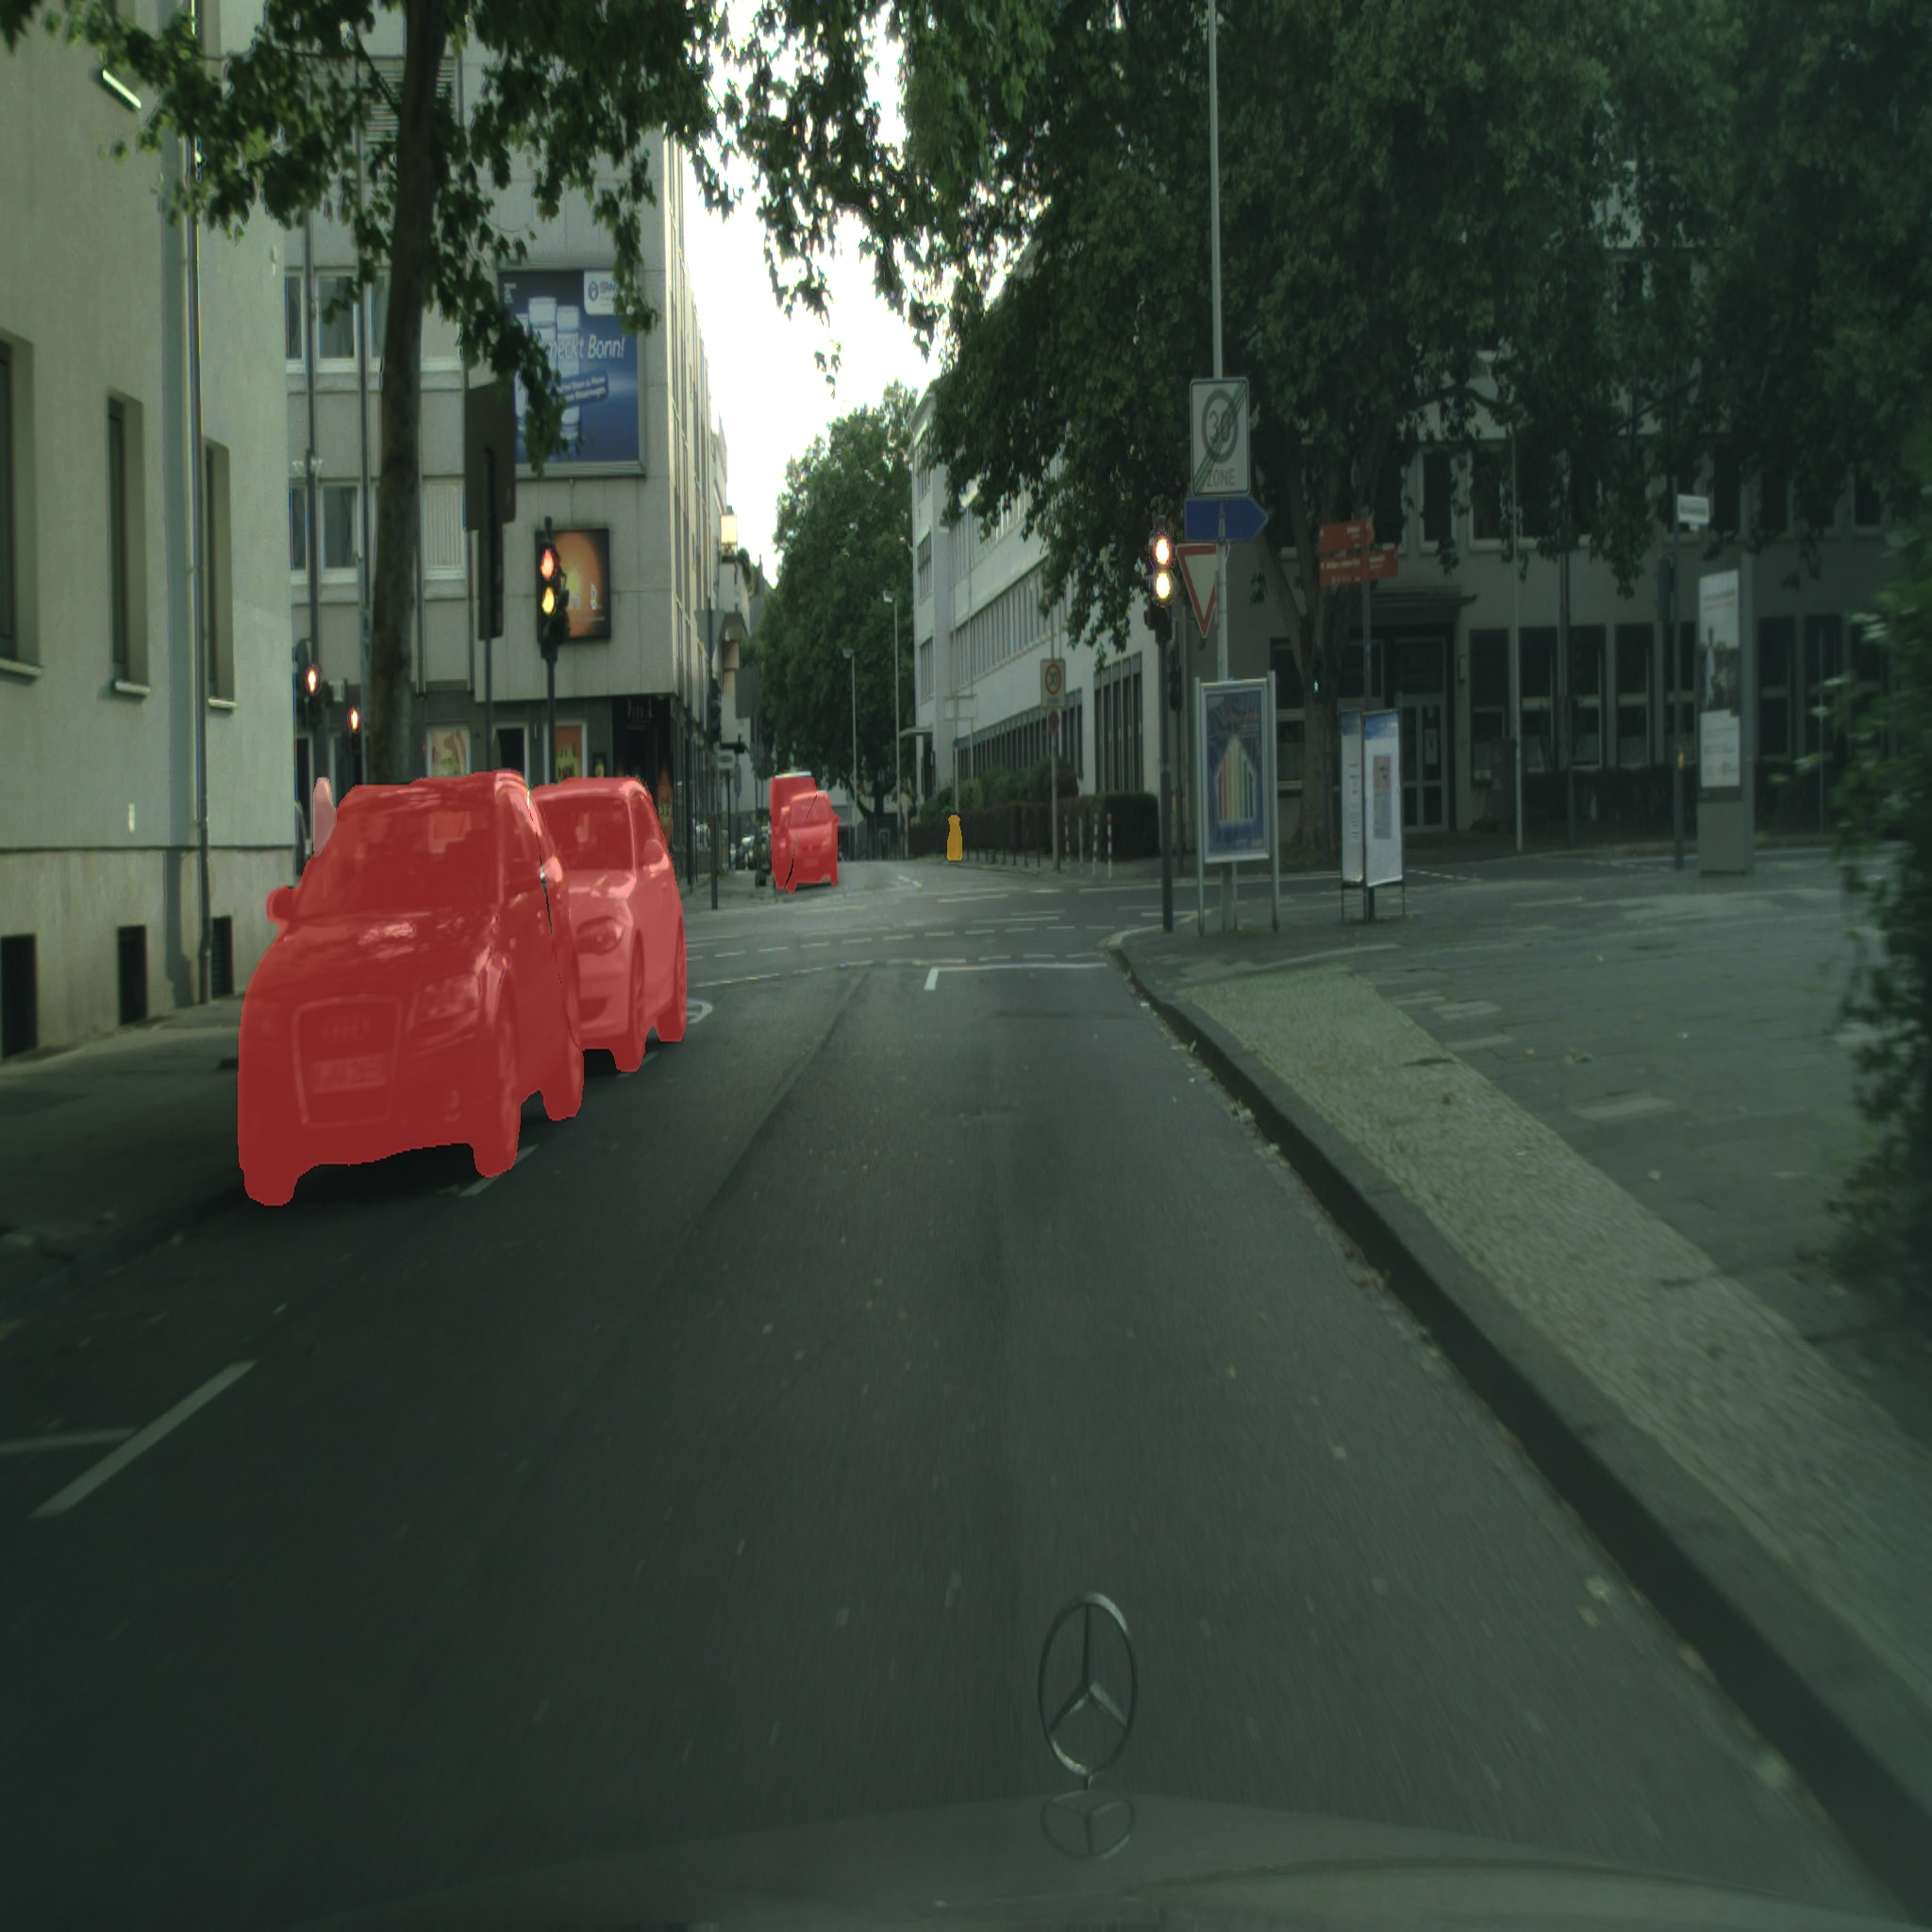
\includegraphics[width=0.316\textwidth]{img} \\
        \hline
        -3.&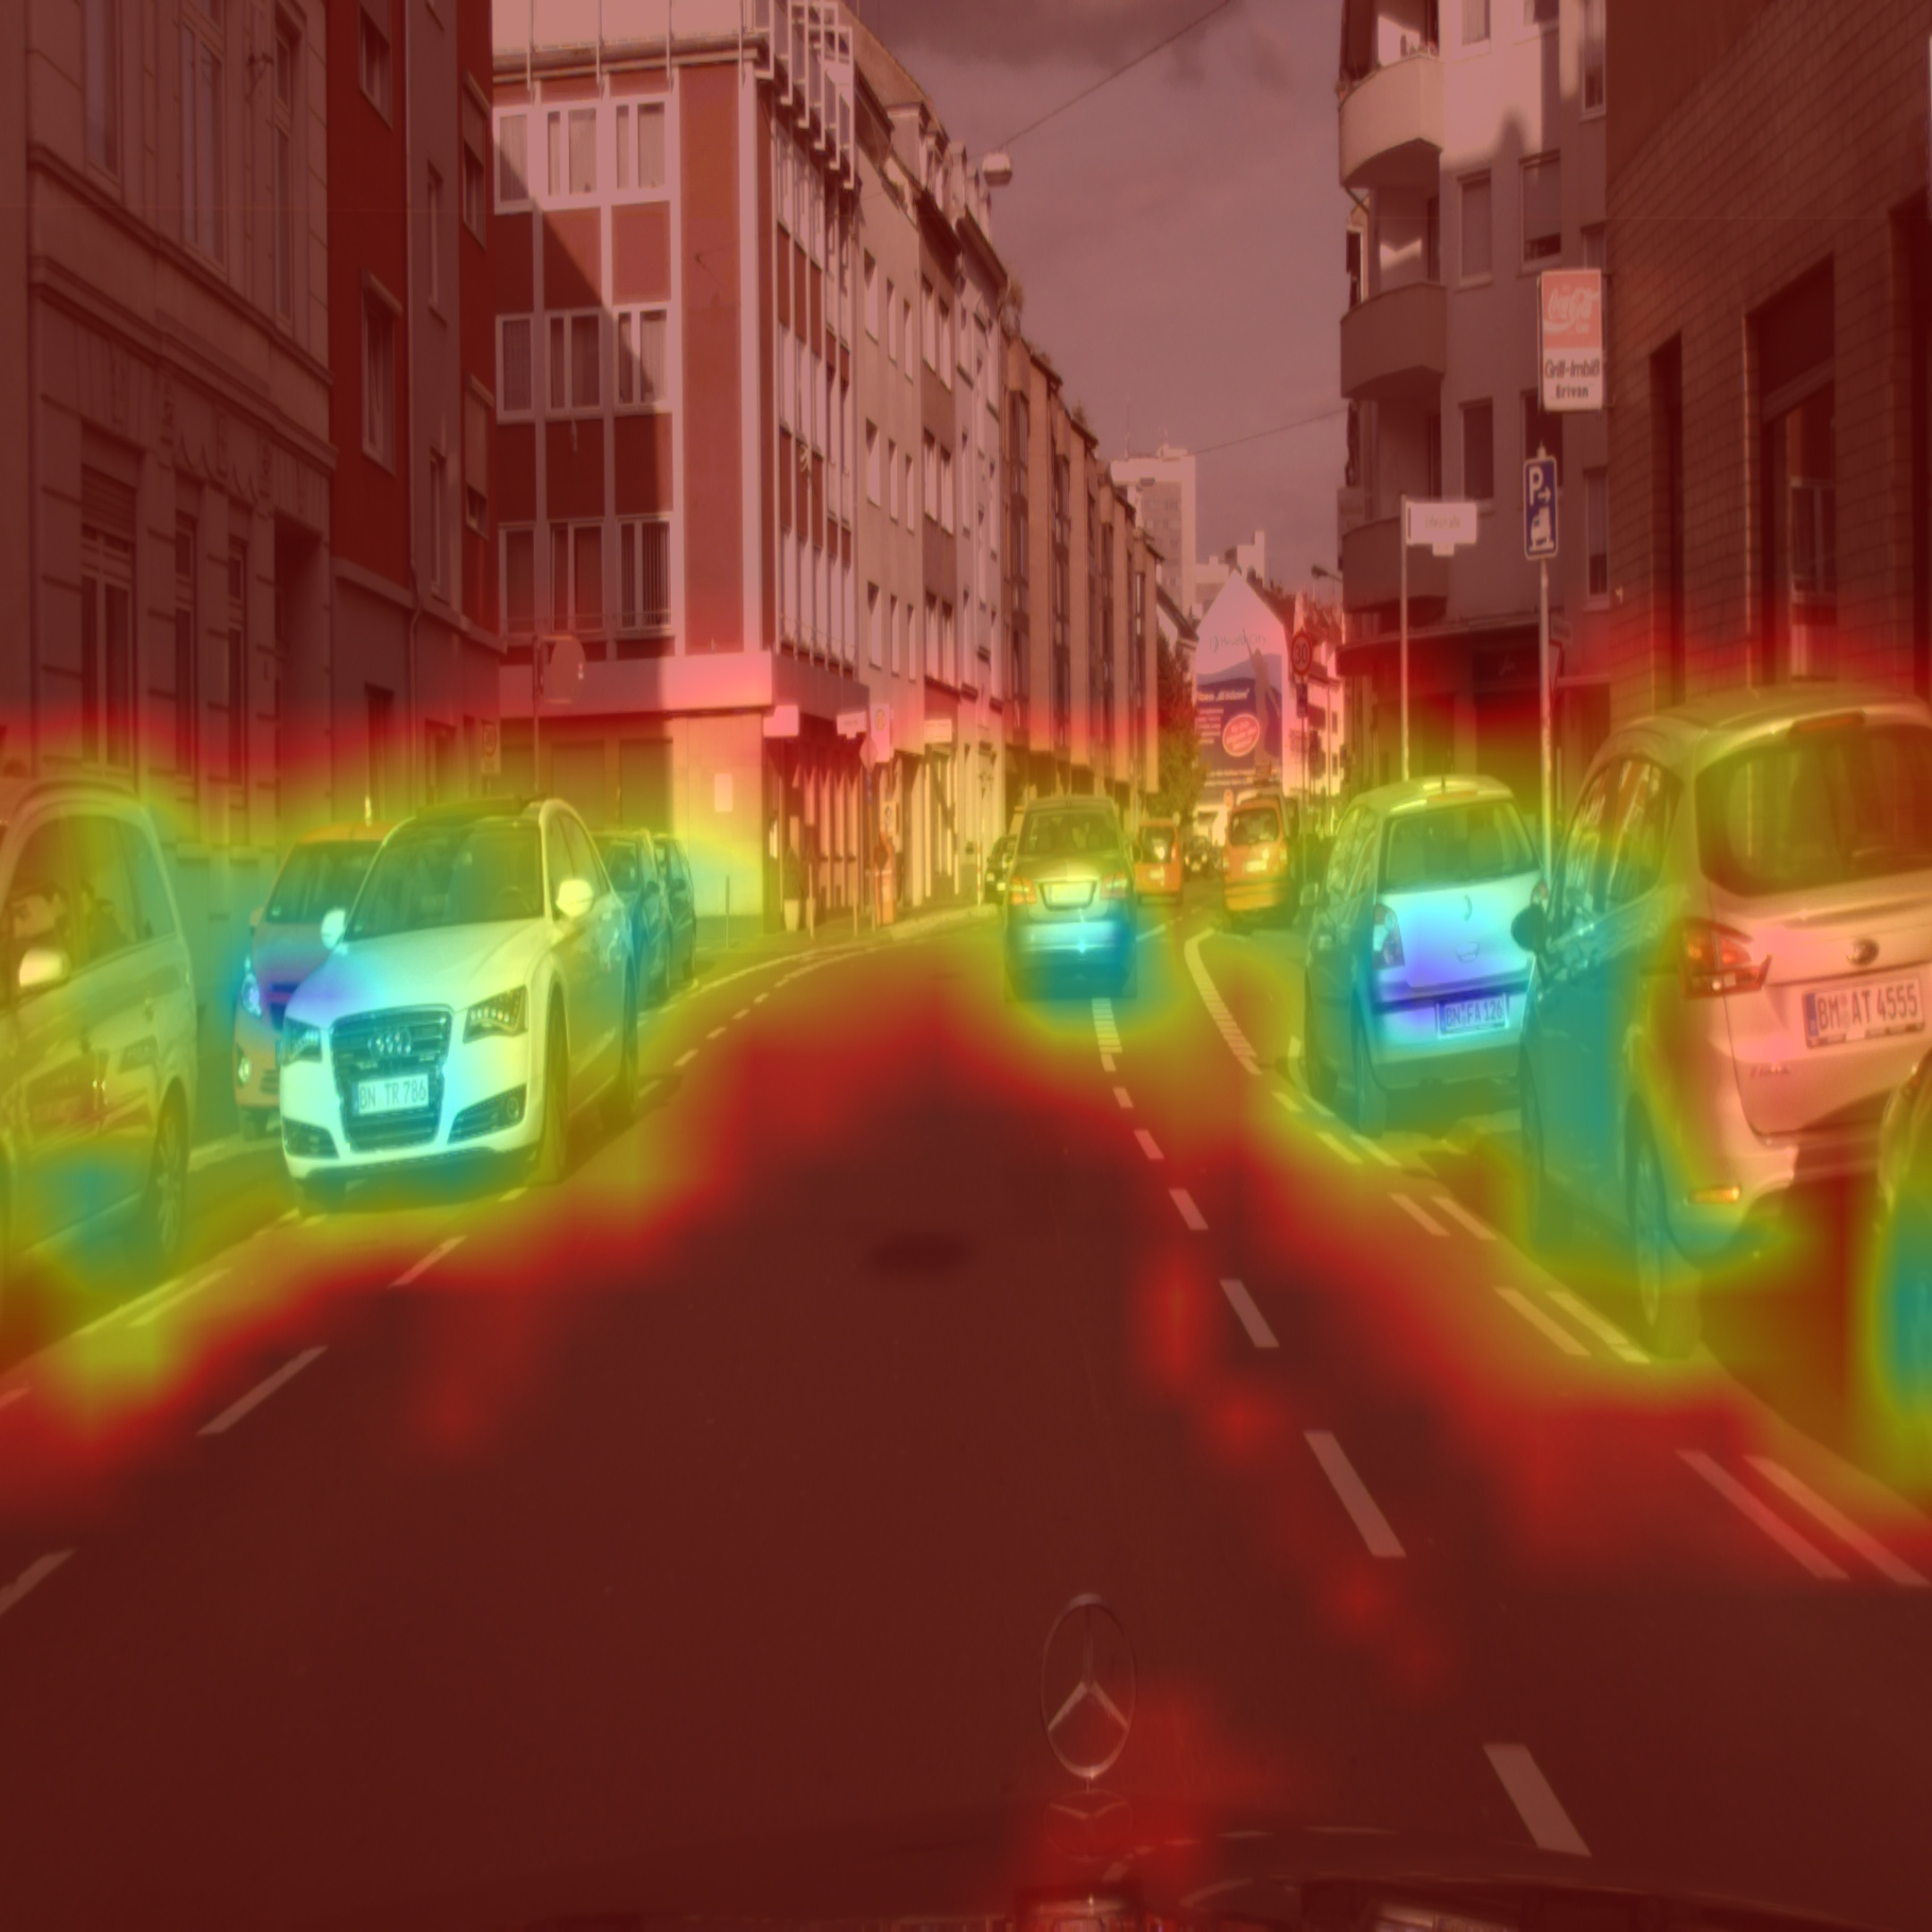
\includegraphics[width=0.316\textwidth]{old_layer-3} &
        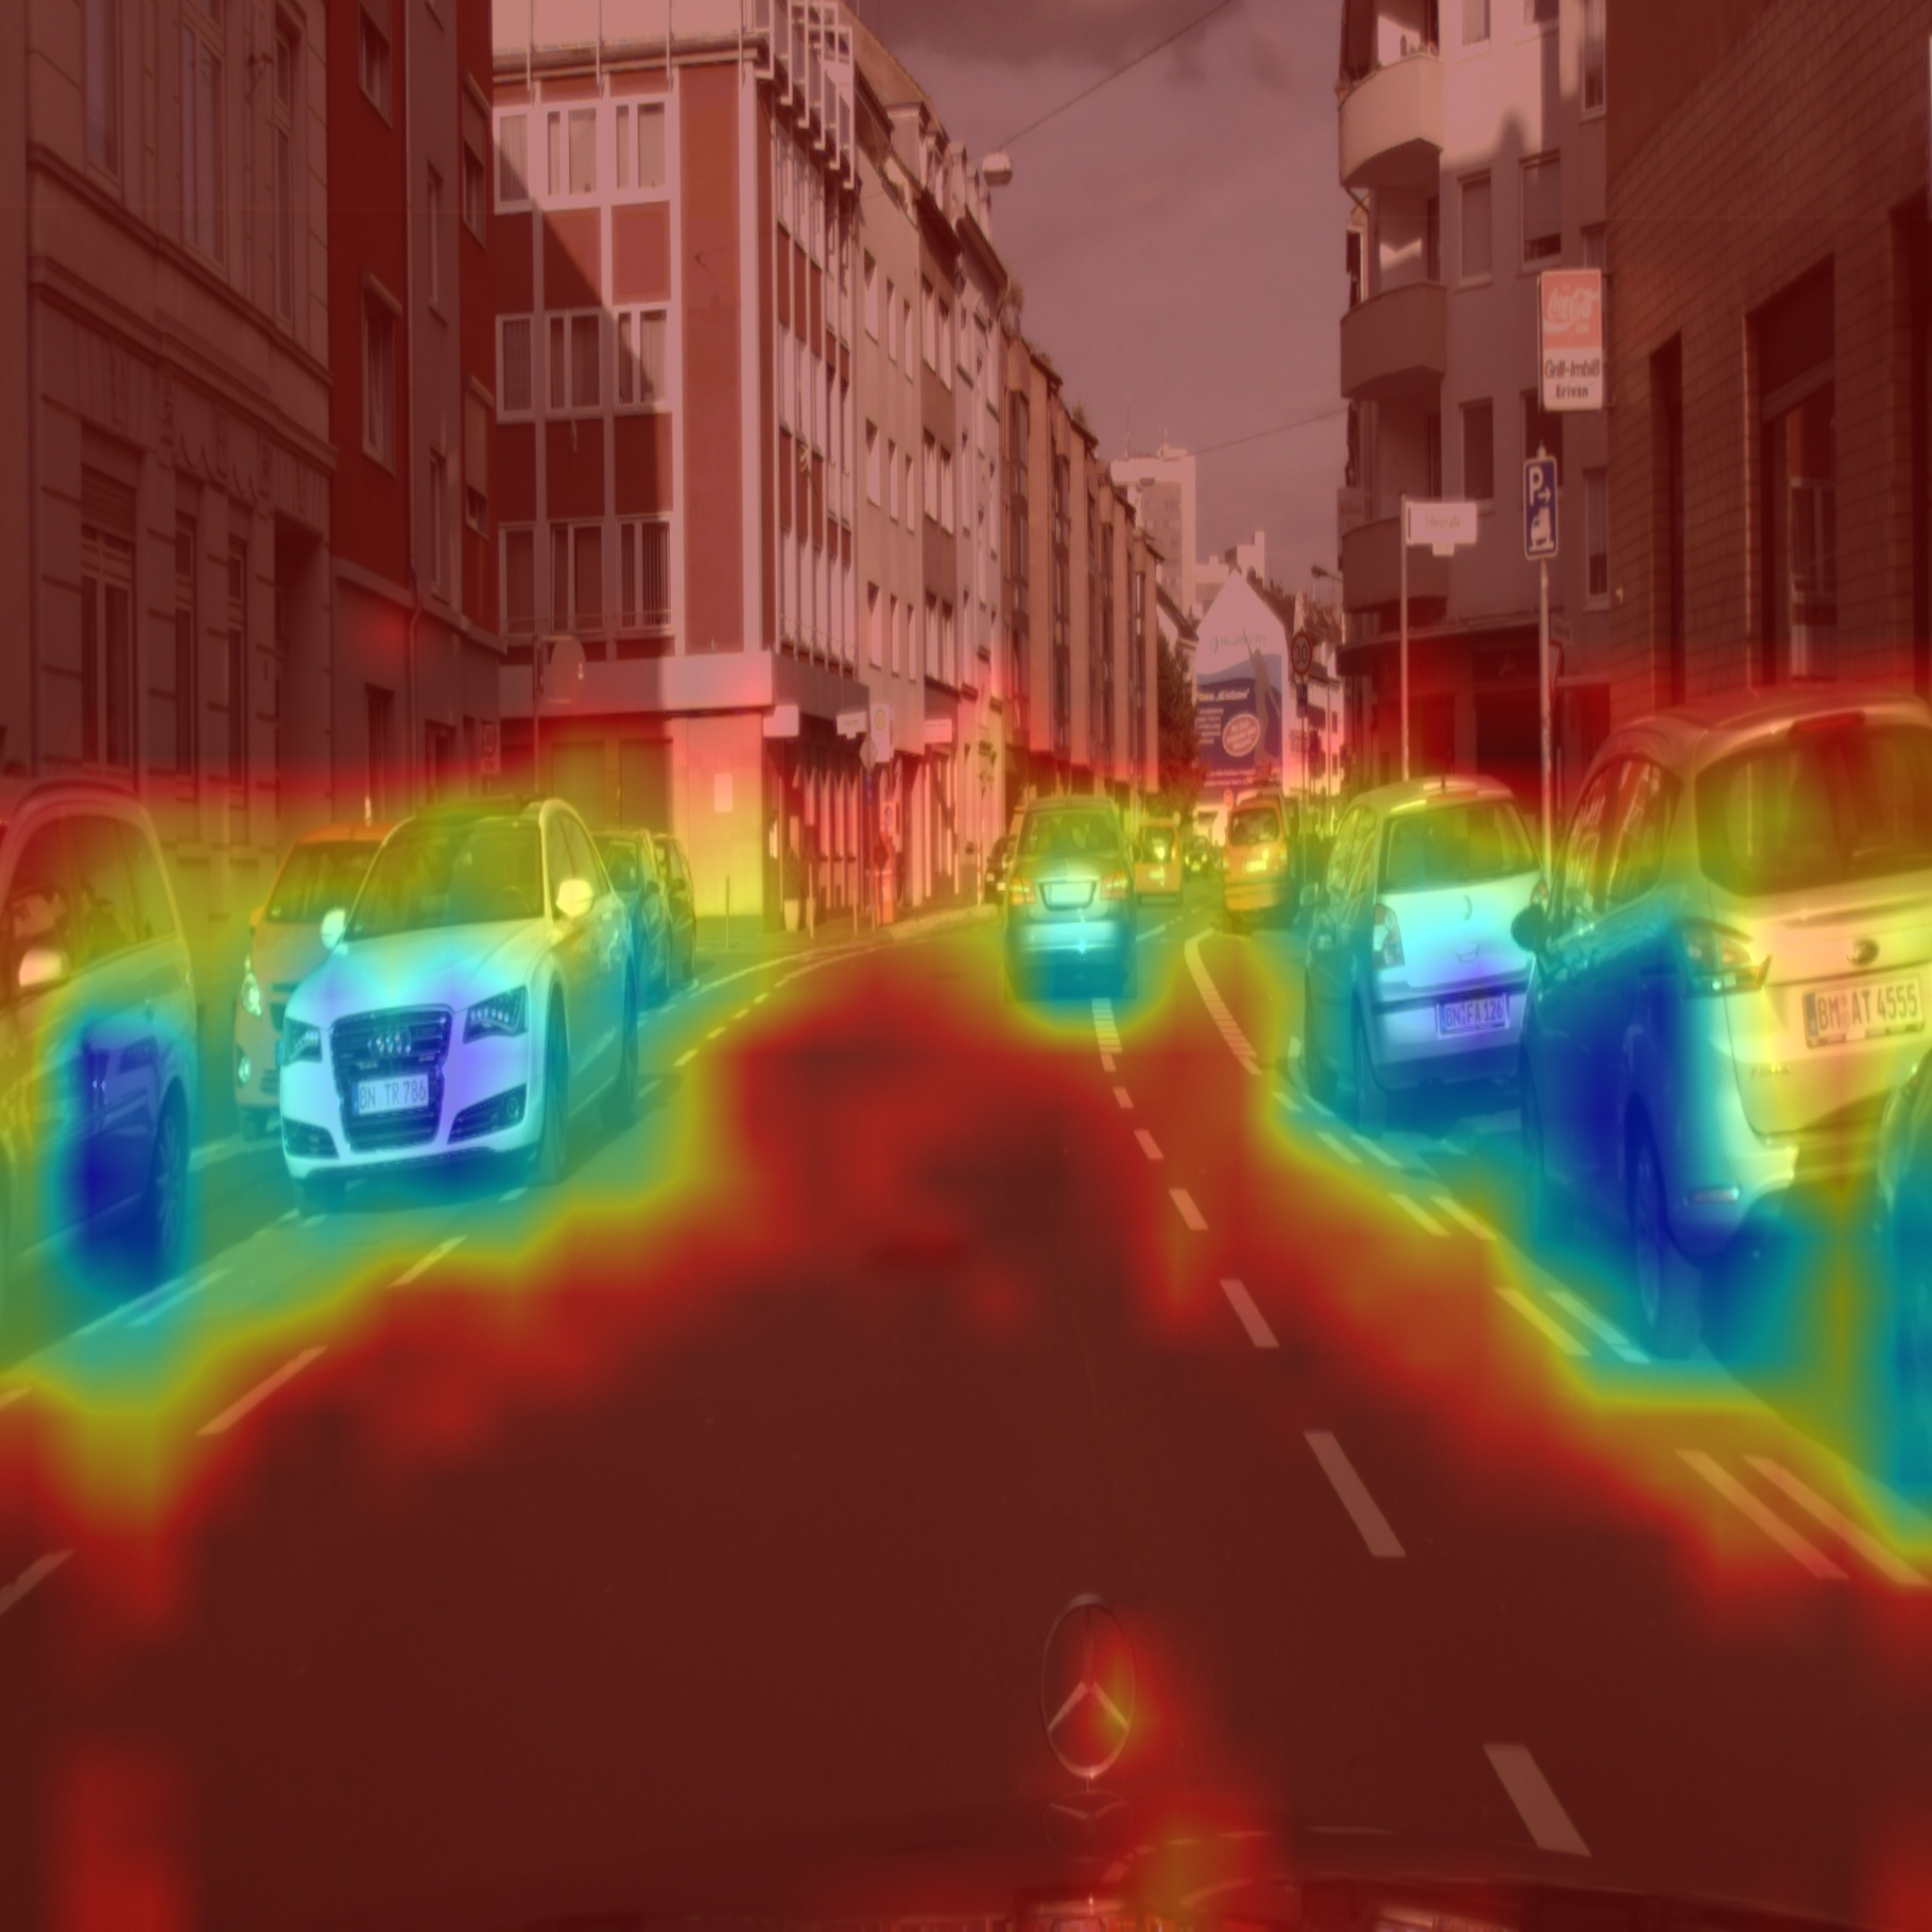
\includegraphics[width=0.316\textwidth]{new_layer-3} &
        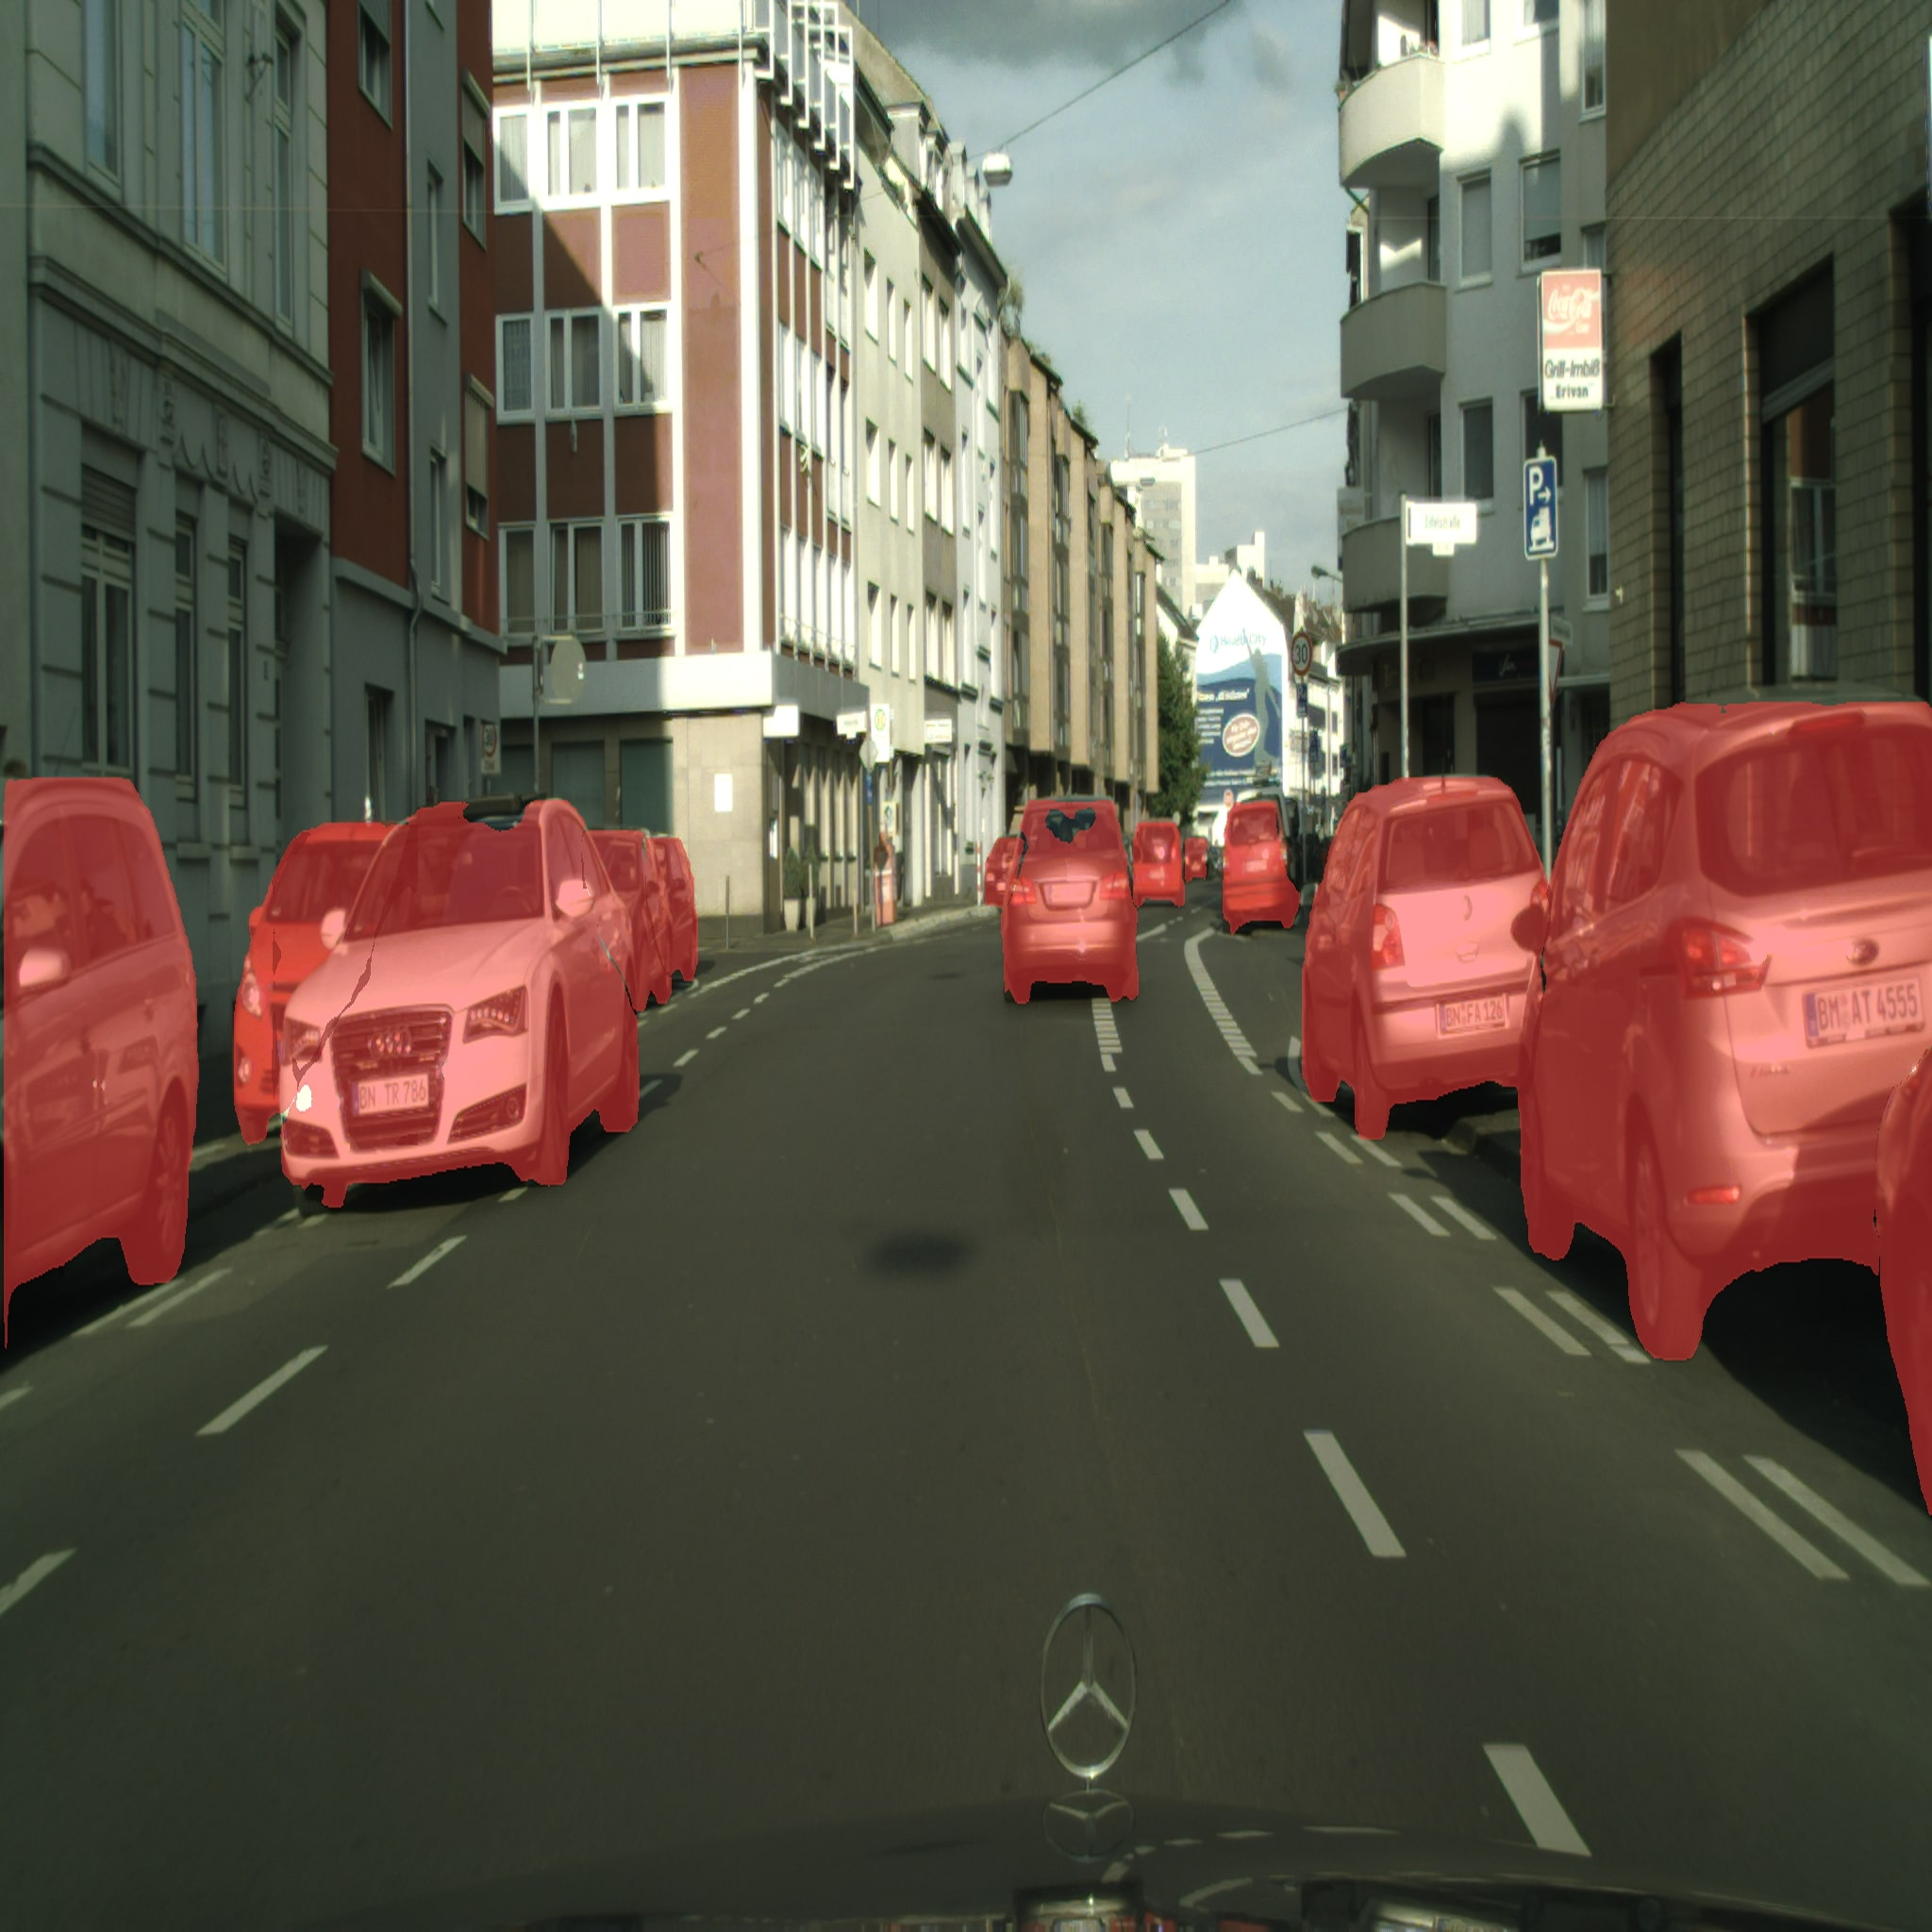
\includegraphics[width=0.316\textwidth]{bonn_000002_000019_leftImg8bit} \\
        \hline
        -2.&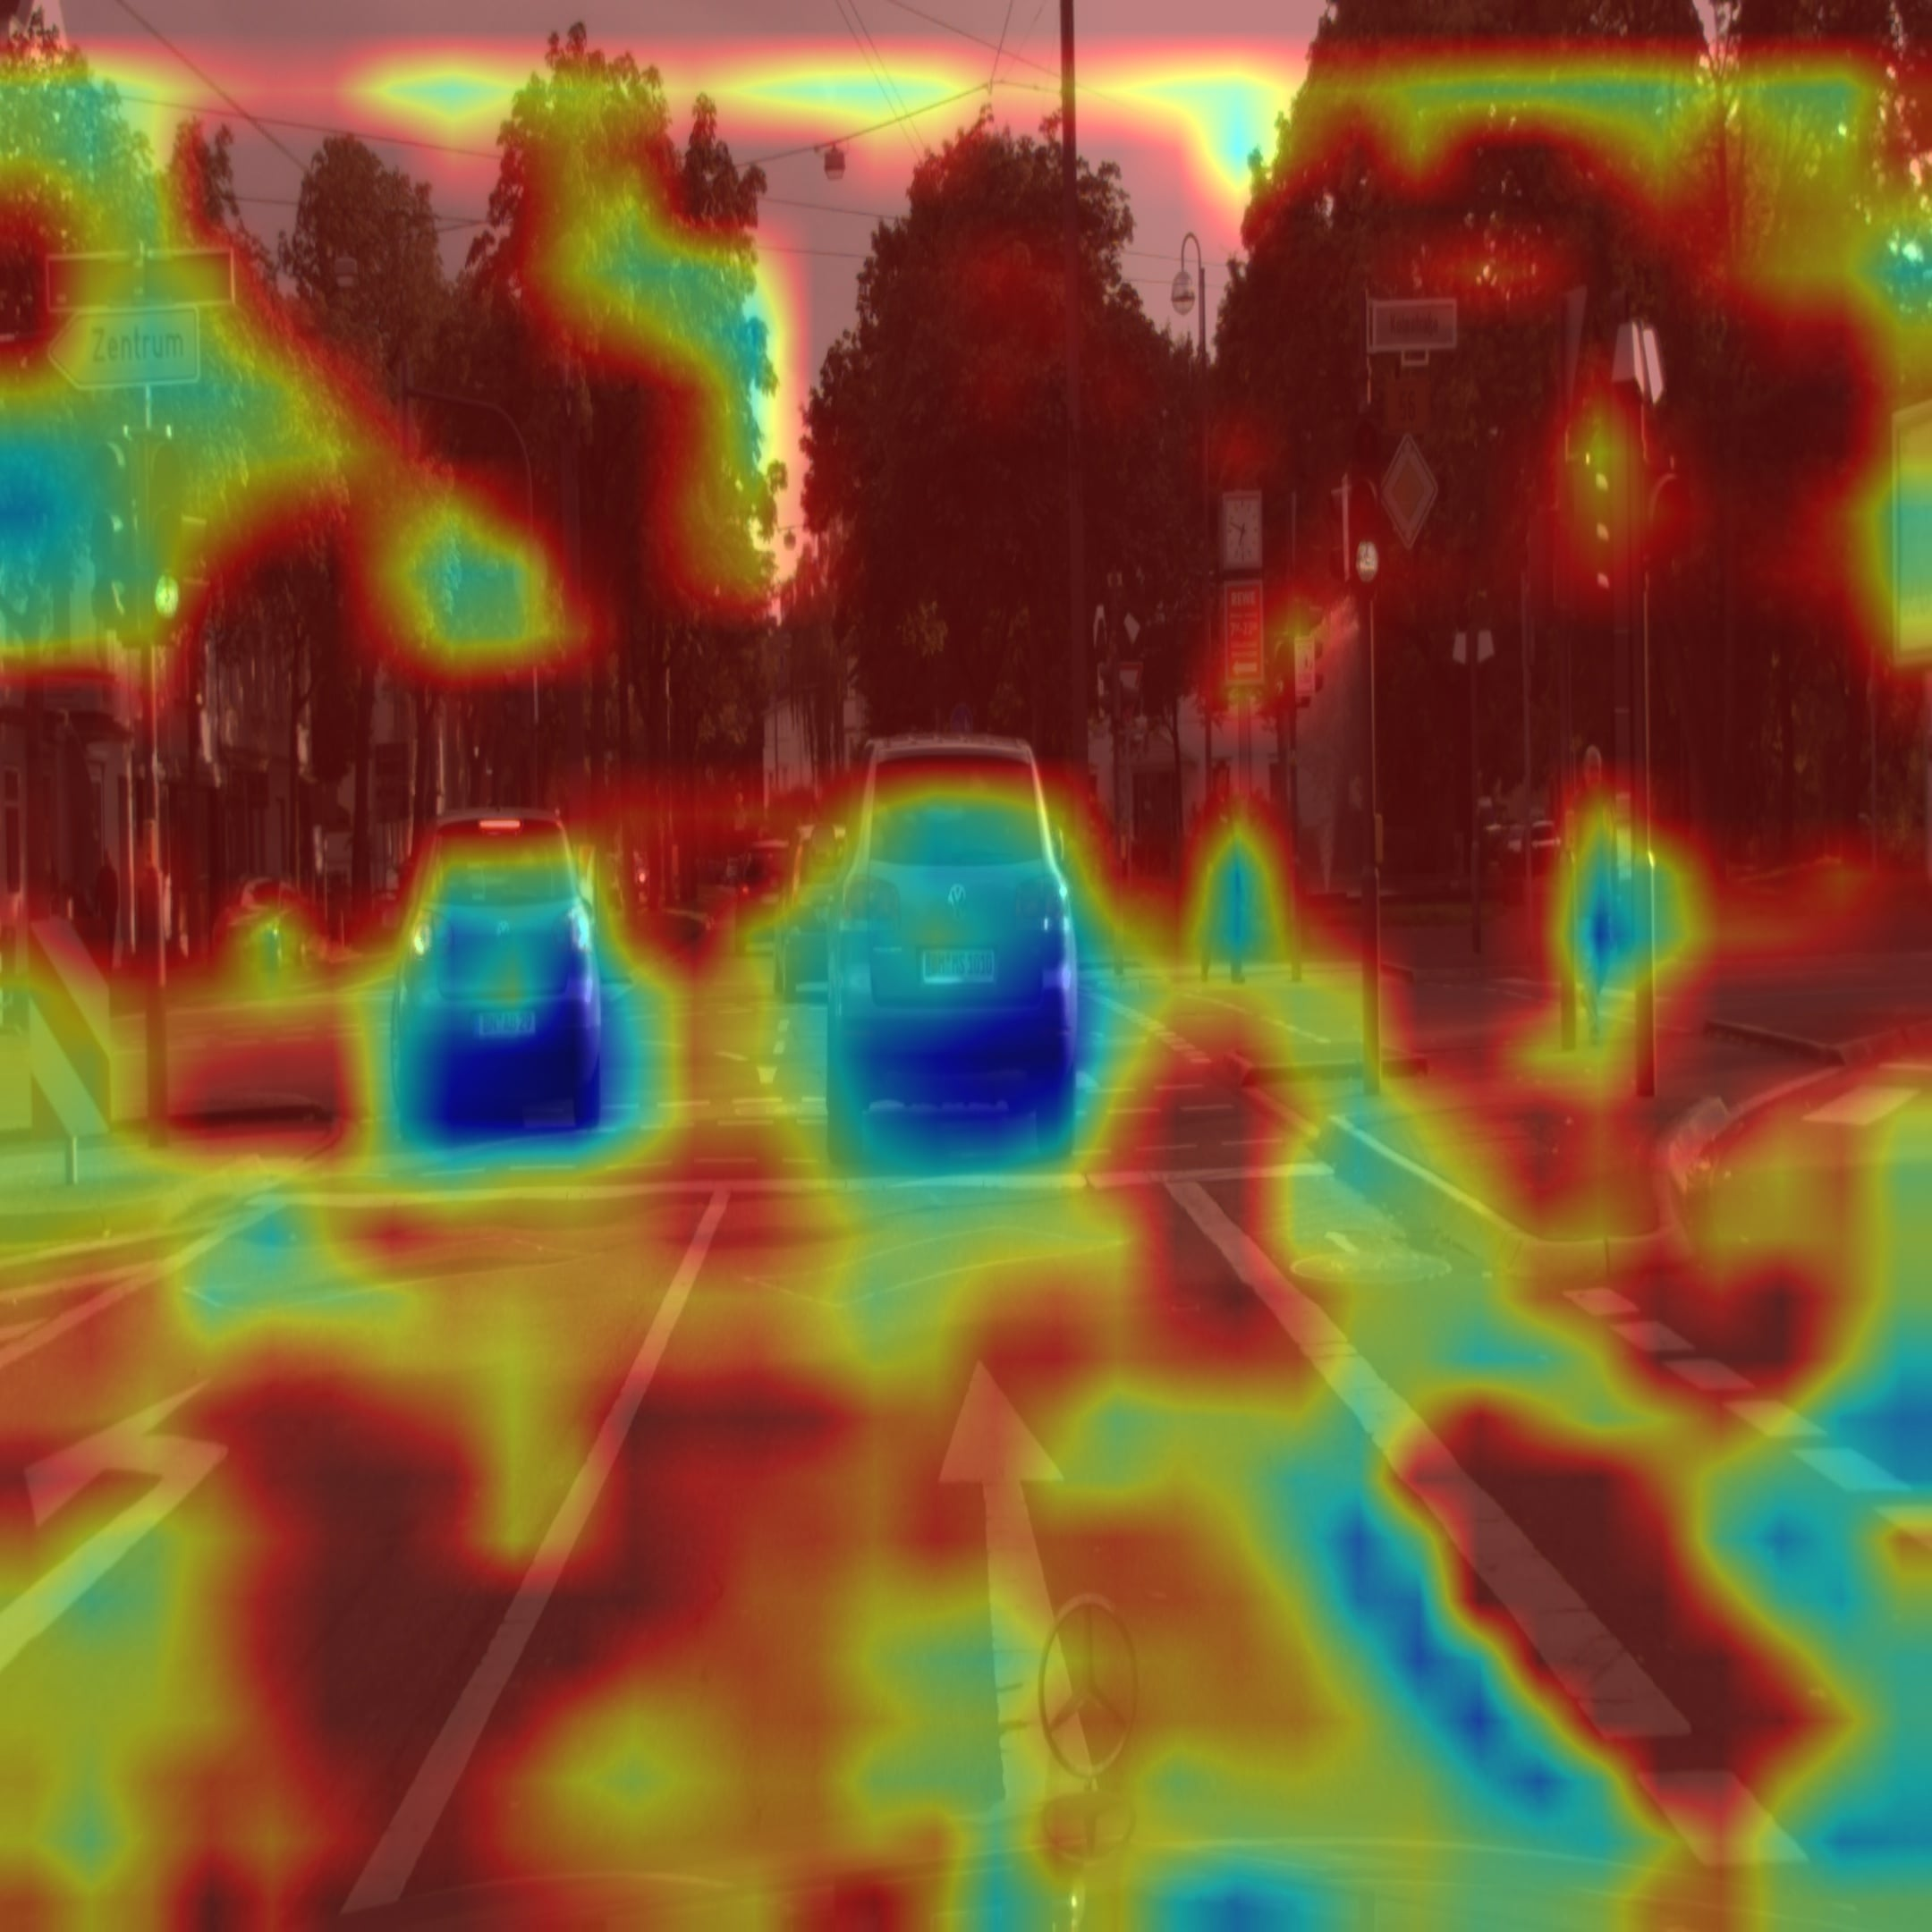
\includegraphics[width=0.316\textwidth]{old_layer-2} &
        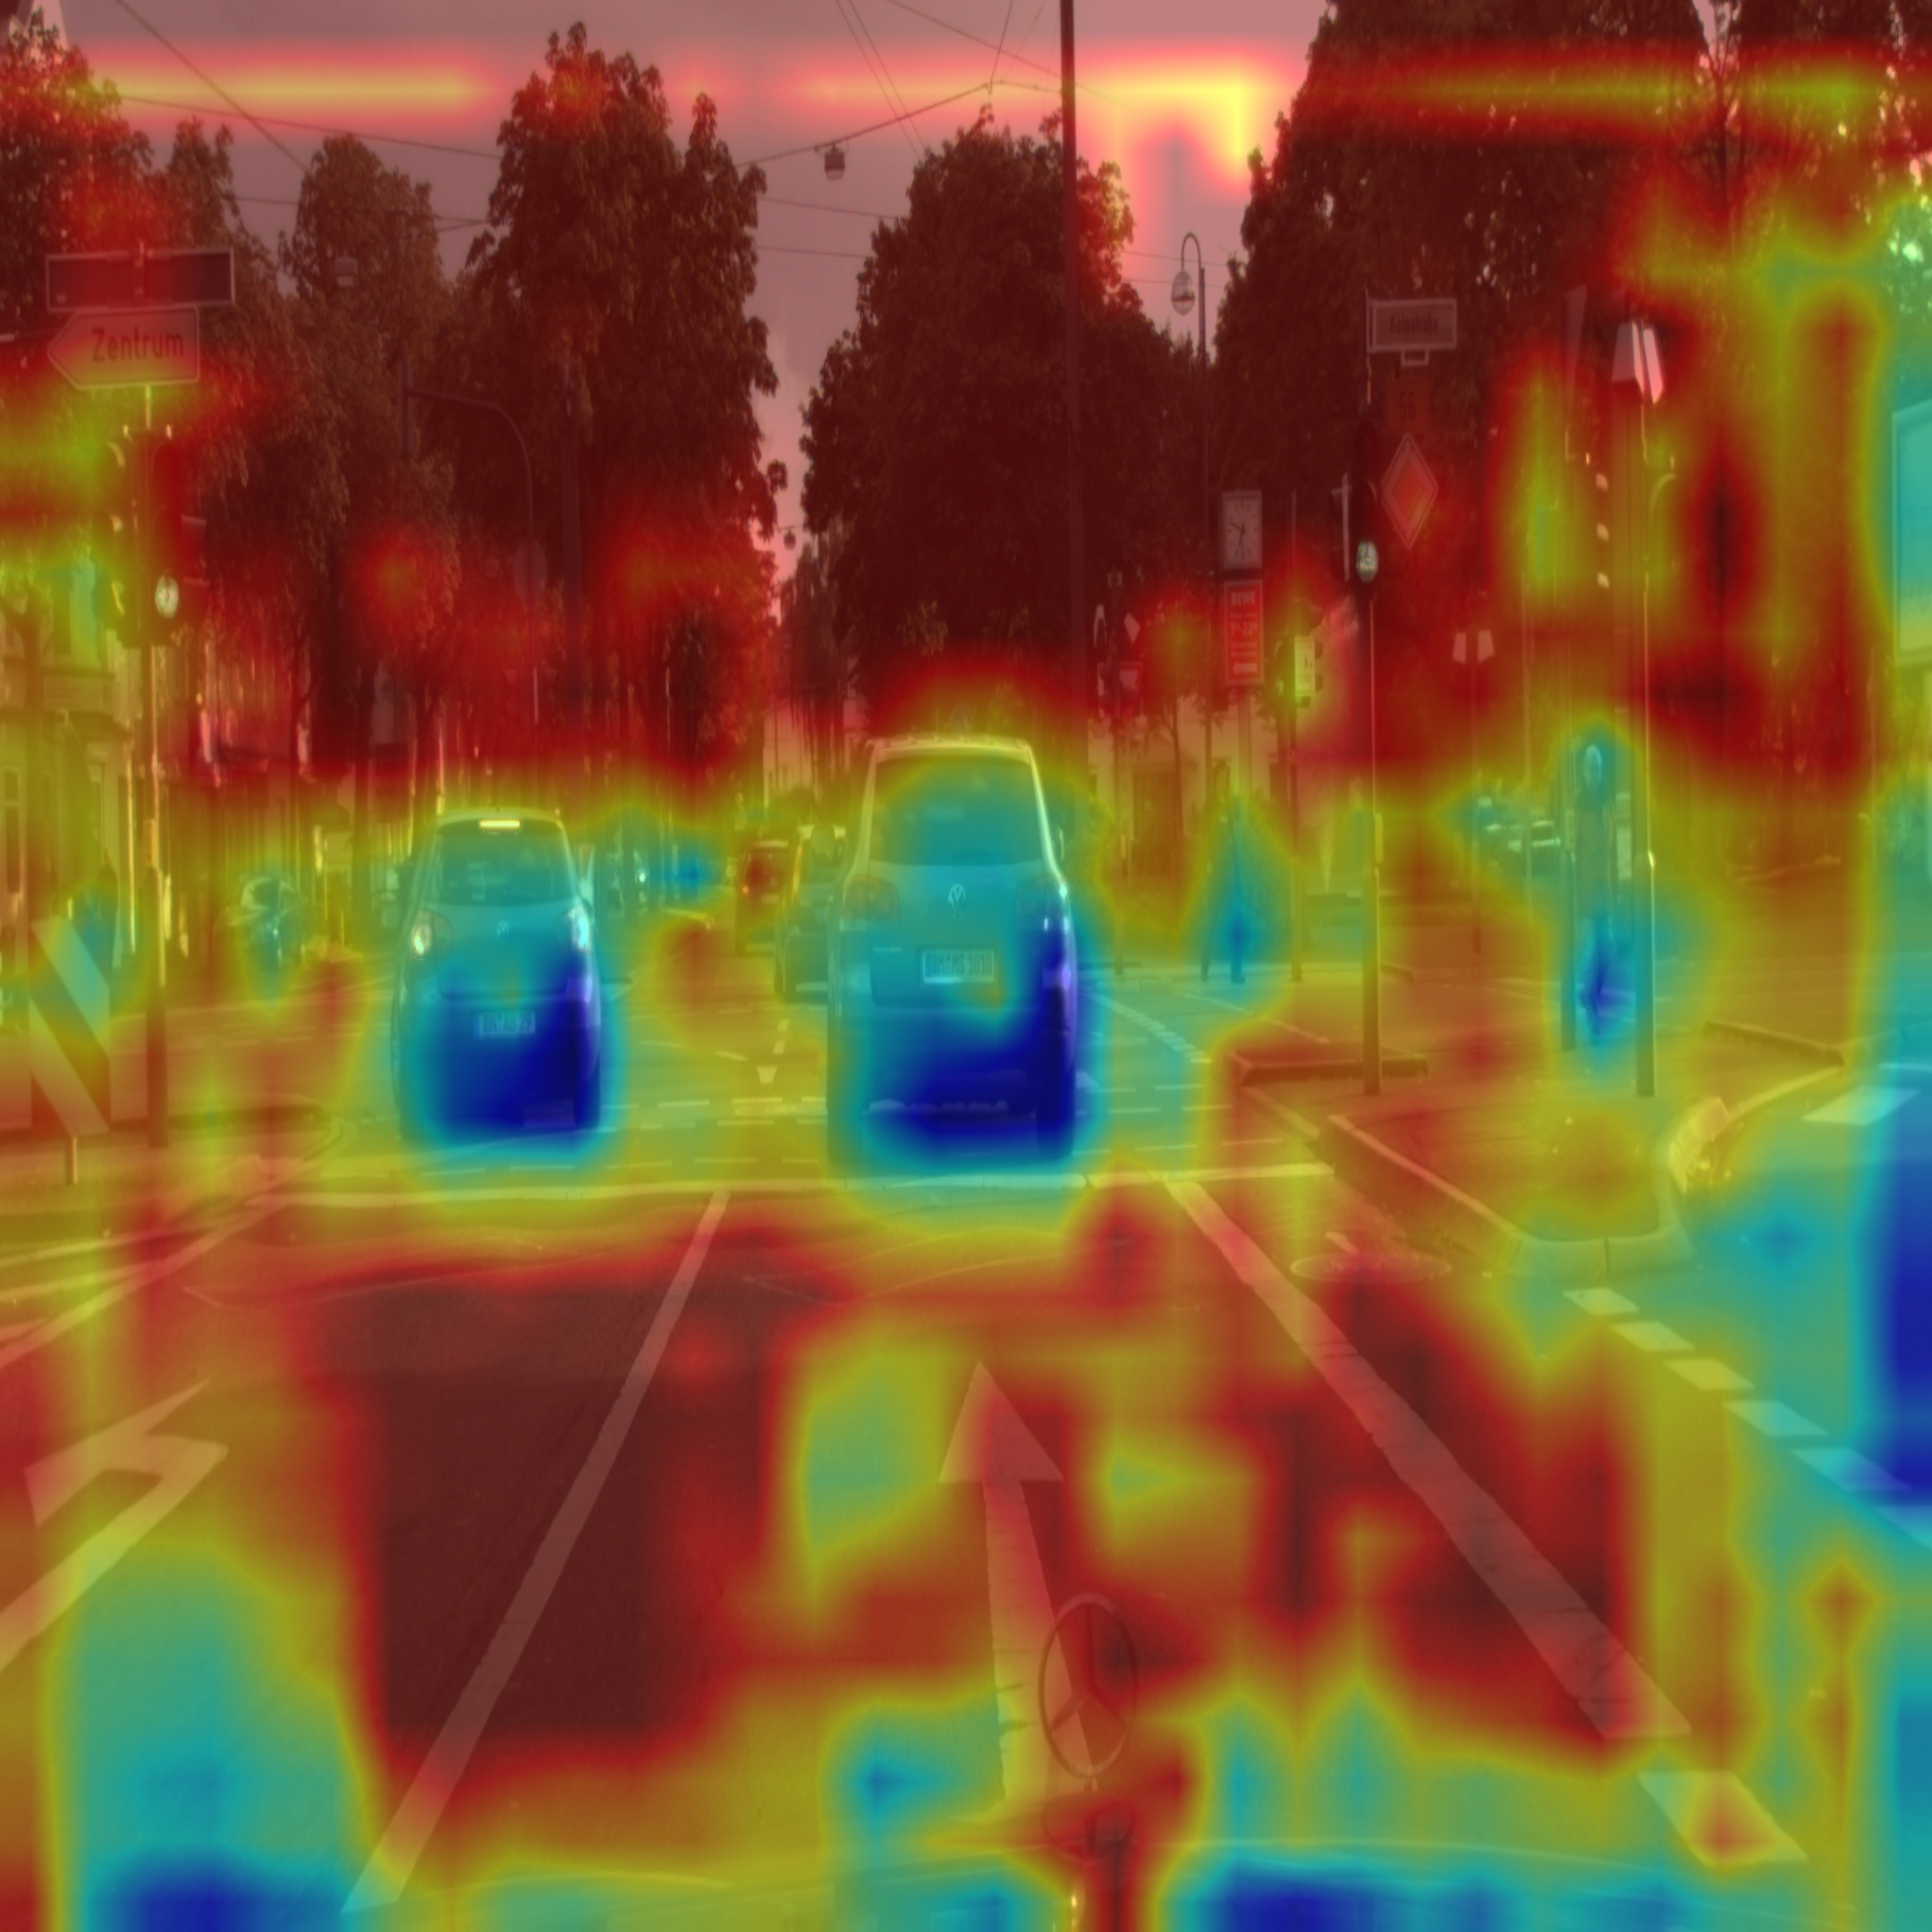
\includegraphics[width=0.316\textwidth]{new_l-2} &
        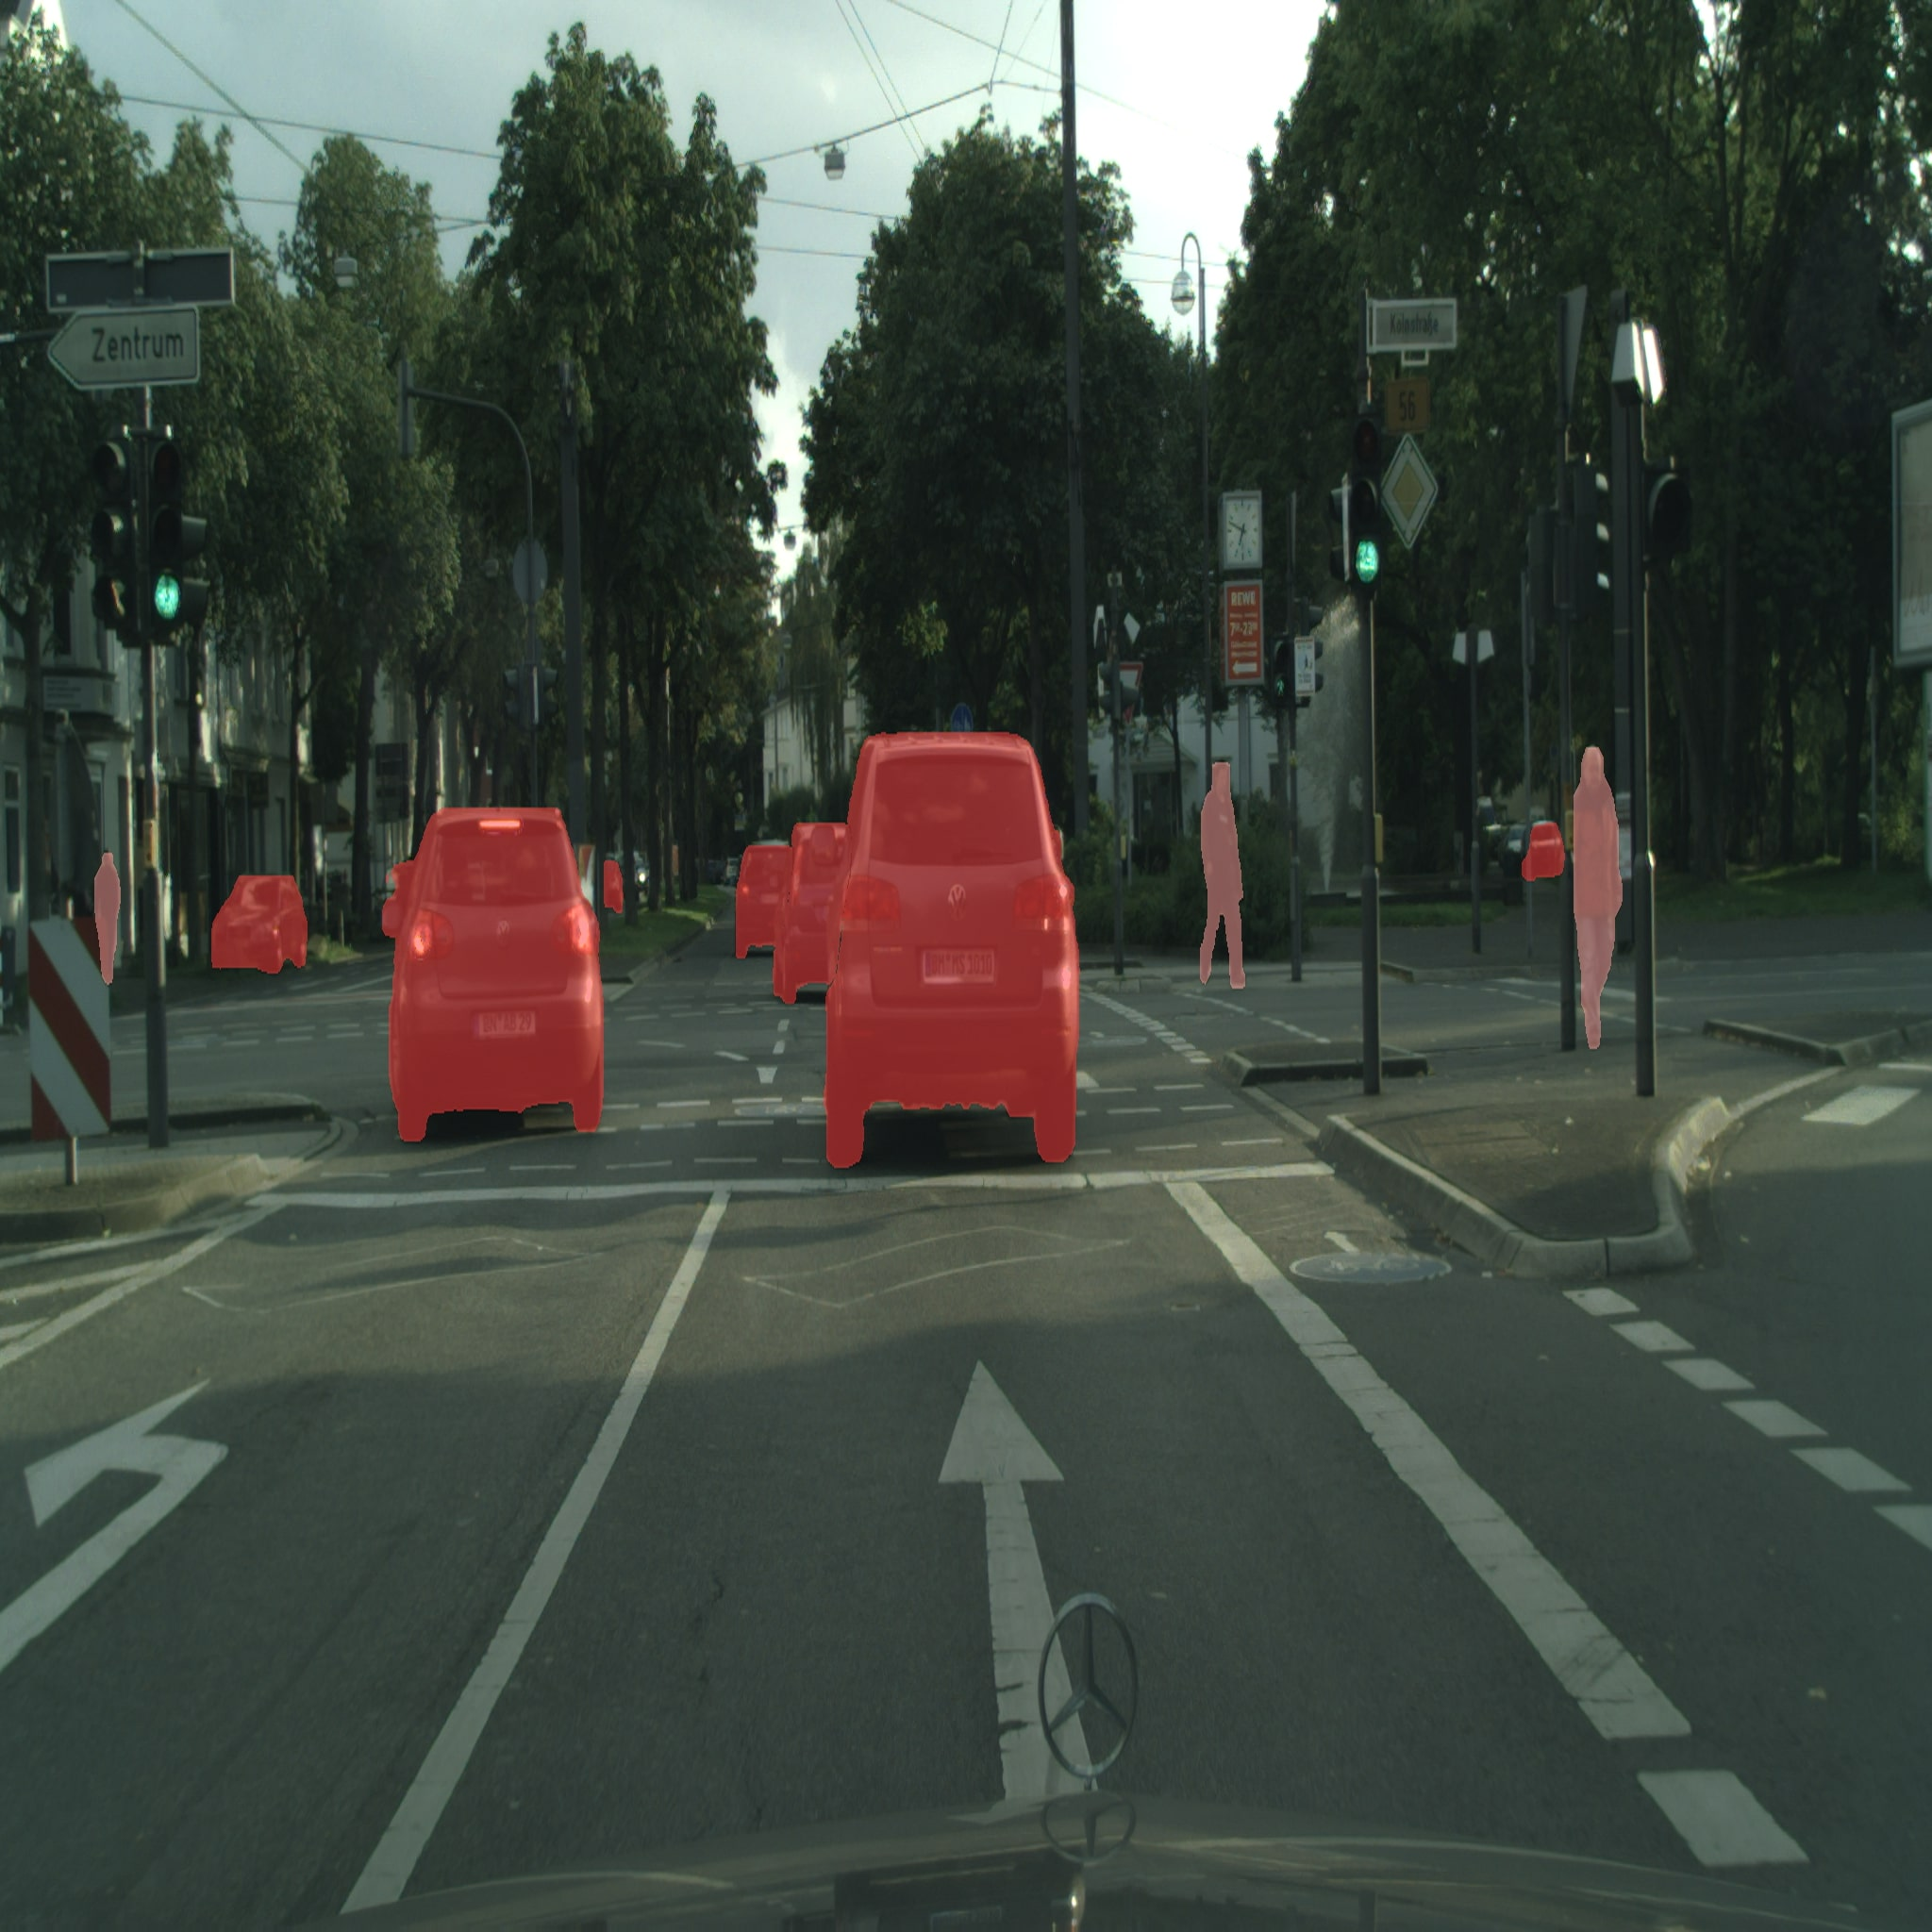
\includegraphics[width=0.316\textwidth]{bonn_000001_000019_leftImg8bit} \\
        \hline
    \end{tabular}
    \caption{Héj aktivációk összehasonlítása a két háló között.}
    \label{tab:Activations}
\end{table}


\subsection{Magyarázat}\label{subsec:magyarazat}
Nem megszokott módon, a heatmapeken az alacsony aktivációs értékeket vöröses árnyalatokkal míg a magas aktivációs értékeket
kékes árnyalatokkal jelölik.

\begin{table}[ht]
    \center
    \begin{tabularx}{\textwidth}{|p{0.07\textwidth}||X|}
        \hline
        \textbf{Layer} & Magyarázat     \\
        \hline
        \textbf{-4}    & Ez a réteg egyetlen konvolúciós réteget tartalmaz.
        Ami nagyrészt éldetekcióval foglalkozik, így az aktiváció nem konzisztensen jelzi a detektálni kívánt osztályokat.
        Inkább élekre aktiválódik amelyek az osztálydetekcióban hasznosak lehetnek ezeket \gls{feature}ökké fogja
        össze és ezeket a \gls{feature}öket továbbítja a következő hálónak.
        Az ennél előrébb lévő rétegek, túl kis méretű \gls{feature}ökkel foglalkoznak és ezek közül sokkal kevesebb lesz használva,
        viszont a sok aktiváció miatt emberi szemmel keveset érthetünk belőle.
        Túl keveset ahhoz, hogy a magyarázhatóság vizsgálatába belevegyem, hiszem emberi szem által nehezen olvasható és érthető.\\
        \hline
        \textbf{-3}    & Ez egy konkatenációs réteg itt a rétegek előzőleg különböző méretű bemeneteket dolgoznak fel.
        Ez a réteg valószínűleg az összes feldolgozott adatot egyetlen tenzorba egyesíti, hogy aztán további
        feldolgozásra kerülhessen.
        Persze az, hogy hol történik \gls{feature} detekció (hol nagyobb az aktiváció) az jól látszik a képeken.
        Ezek a fontos összefűzött \gls{feature}-k
        melyek a következő rétegnek is fontosak lehetnek.\\
        \hline
        \textbf{-2}    &  Ez a réteg konvolúciós rétegeket (cv1 és cv2) tartalmaz, amelyeket egy ModuleList (m) követ,
        amely két Bottleneck blokkot tartalmaz.
        Ezek a blokkok az adatok dimenzióinak csökkentésére és a reprezentációk összeállítására szolgálnak,
        lehetőséget adva az egyszerűbb és hatékonyabb feldolgozásra az utolsó réteg számára.
        Az utolsó héj kimenetei maguk az osztályaktivációk, ezek egyszer sem produkáltak olyan heatmapet amit
        érdemes lett volna vizsgálni, a kijövő kép \("\)horizontális vonalkód\("\) szerű, így azt nem vettem figyelembe a
        magyarázhatósági vizsgálatba.\\
        \hline
    \end{tabularx}
    \caption{Magyarázat}\label{tab:debrief}
\end{table}
Ezen felül az \glsentryshort{EigenCAM} által nyújtott magyarázatokat összehasonlítottam a két hálóra vonatkozóan.
Az \oldh háló kimenetén jól láthatjuk a gyengébb aktivációikat, míg \newh háló centralizált aktivációkat mutat ott, ahol
ténylegesen fel kell ismernie az objektumokat.
Ezen felül még egyértelműen látható, hogy a tanulással arányosan csökken az aktivácók értéke olyan helyeken, ahol csak valamiféle
tetszőleges él található mint például a -4. Layer estében.
Tehát egyértelműen kijelenthetjük hogy a háló tanulását ki tudom mutatni kizárólag csak az aktivációk alapján, az
\glsentryshort{EigenCAM} segítségével.

\newsection{Az EigenCAM alkalmazásának gyakorlati haszna}\label{sec:az-eigencam-alkalmazasanak-gyakorlati-haszna}
    Az \glsentryshort{EigenCAM} és hasonló magyarázó rendszerek alkalmazása esélyt adhatnak nekünk arra, hogy esetekre
    , tehát egyéni bemenetekre (a képfelismerés esetében ezek a képek), vonatkozó döntéseihez a kép milyen részei
    milyen fontossággal asszisztáltak.
    Lehet értelmezni a háló architektúrájának tudatában, hogy éppen melyik réteg milyen információt dolgoz fel
    és ezekből milyen hiedelmeket (értelmezett információkat) alkot.
    Érdekes az is, hogy mint ahogy~\pageref{subsec:magyarazat}. oldalon láthattuk a háló tanulását is meg tudjuk
    figyelni az aktivációk alapján és ebből következtetéseket tudunk levonni arra vonatkozóan, hogy mik alapján észlelik
    az objektumokat, kiküszöbölve olyan hibákat, amelyeket a korai mesterséges intelligencia  alapú
    \ac{CV} szoftverek tartalmazhattak, például a háttér túlzott befolyása az objektum osztályának meghatározásában.

\subsection{Eredmények összegzése}\label{subsec:osszegzes-es-kovetkeztetes}
    % Összefoglalás az EigenCAM és a YOLOv8 magyarázhatóságáról.
    % Fontos tanulságok és a jövőbeli munkák összefoglalása.
    Féléves munkámban tehát a \glsentryshort{EigenCAM} modellmagyarázó módszert és a \glsentryshort{Yolov8}
    szemantikus szegmentációs háló interpretálhatóságát vizsgáltam valamint feladatom volt az adat előkészítése és elemzése is.

    Az \glsentryshort{EigenCAM} segítségével vizualizáltam az aktivációkat, és kísérletet tettem a hálók működésének megértésére.
    Ezáltal figyelhettem meg a háló tanulását: mit jelenthet adott esetben a túltanulás fogalma és azt, miben is
    különbözik egy háló aminek jobb az \("\)Accuracy\("\) és a \("\)Recall\("\) mutatója is, egy másik ugyanazon az adaton és
    osztályokra tanított, ugyanolyan architektúrájú hálótól.

    Ezen felül foglalkoztam az új architektúrával, Yolov5-ről Yolov8-ra tértem át, és először használtam felhő alapú
    MLOps megoldásokat munkám segítésére, mint például a Comet (\url{https://www.comet.ml}) amelyben \aref{subsec:MLOps} fejezetben
    részleteztem.

\newsection{Jövőbeli irányok és kutatási lehetőségek}\label{sec:jovobeli-iranyok-es-kutatasi-lehetosegek}
    % Lehetséges fejlesztési irányok az EigenCAM és a YOLOv8 interpretálhatóságának javítására.
    % Új kutatási lehetőségek a mély tanuló modellek magyarázhatóságának területén.
    A \glsentryshort{Yolov8} neurális háló most is vezető szerepet élvez az autóipari szolgáltatásokban képfelismerés
    témakörében.
    Azon belül a szemantikus szegmentációban\index{szemantikus szegmentáció}, ami az elmúlt években előnyt élvez
    a hagyományos  két- és háromdimenziós keretekkel szemben, a kereteknél jóval nagyobb pontossága
    és a maszkok által hordozott temérdek információ gazdagsága miatt.

    A következőkben tehát a jelenlegi munkámban még a kezdetlegesebb, kiforratlanabb módszert, a modellmagyarázást
    (vagyis Explainable AI-t
    \ac{XAI}) szeretném továbbfejleszteni.
    Mivel a jelenlegi megoldásom modellfüggő és héjaktiváció-alapú, nem vesz figyelembe gradienseket,
    valamint érzékeny a modell belső felépítésére is.
    Célom a jövőben a modellek tanulásának folyamatát figyelni más módszerekkel is, amellyek például a héjjak gradienseit
    figyelembe veszik, azért hogy a magyarázataik pontosabbak, rendszerszerűbbek és megbízhatóak legyenek.
    A következő konkrét tervet határoztam meg további munkámhoz:
    \begin{enumerate}
        \item Lime vagy Shap módszerek behozása és összehasonlítása az EigenCAM-mal.
               \cite{ribeiro-etal-2016-trust,lundberg2017unified}
        \item EigenGradCAM bevezetése a modell tanulásának folyamatának figyelembevételére.
    \end{enumerate}


\printindex\label{ossz:indexjegyzek}

\newsection{Szó- és rövidítés jegyzék}\label{sec:szó-es-rövidités-jegyzék}
\printglossary\label{ossz:glossary}
\newpage
\subsection{Rövidítésjegyzék}\label{subsec:röviditésjegyzék}
\begin{acronym}\label{ossz:roviditesjegyzek}
    \acro{EU}{Európai Únió}
    \acro{GDPR}{Általános Adatvédelmi Rendelet}
    \acro{CV}{Computer Vision}
    \acro{XAI}{Explainable AI}
    \acro{MLOps}{Machine Learning Operation}
    \acro{ML}{Machine Learning}
    \acro{mAP}{Mean Average Precision}
    \acro{IoU}{Intersection over Union}
    \acro{ReLU}{Rectified Linear Unit}
    \acro{LReLu}{Leaky Rectified Linear Unit}
    \acro{ms}{miliszekundum}
\end{acronym}
\newpage
\bibliographystyle{plain}
\bibliography{bibliography}\label{ossz:irodalomjegyzek}


\begin{table}[ht]
    \center
    \begin{tabular}{|lc|}
        \hline
        Formai elem                            & Megvalósítás                                                             \\
        \hline
        irodalomjegyzék                        &~\hyperref[ossz:irodalomjegyzek]{itt} \\
        tartalomjegyzék                        &~\hyperref[ossz:tartalomjegyzek]{itt}  \\
        rövidítésjegyzék                       &~\hyperref[ossz:roviditesjegyzek]{itt}  \\
        indexjegyzék                           &~\hyperref[ossz:glossary]{itt}        \\
        táblázat                               &~\hyperref[tab:Activations]{itt} és~\hyperref[tab:debrief]{itt}\\
        hivatkozás táblázatra                  &~\hyperref[hivatkozas]{itt} \\
        vektor-grafikus kép                    &~\hyperref[fig:Ultralytics]{itt}  \\
        raszter-grafikus kép                   &~\hyperref[fig:CityScapes-Examples]{itt}  \\
        hivatkozás képre                       &~\hyperref[kephivatkozas]{itt} \\
        tikz ábra                              &~\hyperref[fig:flowchart]{itt}  \\
        hivatkozás ábrára                      &~\hyperref[abrahiv]{itt}         \\
        képlet                                 &~\hyperref[eq:LRELU]{itt}      \\
        hivatkozás képletre                    &~\hyperref[eqhivatkozas]{itt}         \\
        képletcsoport                          &~\hyperref[eq:activation_functions]{itt}\\
        hivatkozás képletcsoport egy képletére &~\hyperref[alignhivatkozas]{itt} \\
        fejezet                                &~\hyperref[sec:bevezetes]{itt}    \\
        hivatkozás fejezetre                   &~\hyperref[sechiv]{itt}     \\
        lista                                  &~\hyperref[itemize]{itt}     \\
        hivatkozás lista elemre                &~\hyperref[listahiv]{itt}     \\
        hivatkozás oldalszámra                 &~\hyperref[pageref]{itt}       \\
        hivatkozás irodalomra                  &~\hyperref[irodalomhivatkozas]{itt}\\
        saját makró használata                 &~\hyperref[makrohasznalat]{itt}       \\
        \hline
    \end{tabular}\label{tab:table}
\end{table}

\end{document}
